\chapter{Results and Discussion}
\label{chap:exp}
This chapter presents the experimental results of the proposed \ac{DBN} framework and discusses the effect of the main modeling choices. 
The goal of the study is to identify which configuration provides the best trade-off between generative fit, predictive usefulness, and model complexity.

\par All compared models use the same preprocessing pipeline, the same vehicle-level train/validation/test split, the same window-based observation representation, 
and the same \ac{EM}-based training procedure described in \autoref{chap:methodology}. 
The compared settings differ mainly in the emission-model formulation, the treatment of the initial latent-state distribution, the use of lane-change weighting scheme, 
and the inclusion of Bernoulli likelihood terms.

\par In addition to these core comparisons, a set of latent-cardinality ablation studies is also carried out. 
These ablations vary the number of style and action states in order to assess whether the selected latent structure is appropriate for the prediction task. 
Besides the main setting with two style states and four action states, additional variants such as 2S3A, 2S5A, 1S4A, and 1S5A are evaluated. 
These experiments help determine whether the style variable is beneficial and whether increasing the number of action states leads to a more useful behavioral decomposition.


\section{Main S2A4 Configuration Study}
\label{sec:main_s2a4_study}
The main study considers the setting with two style states and four action states. 
This choice is based on the assumption that two latent behavioral styles are sufficient to represent the dominant driver regimes.
Within this S2A4 setting, 24 configurations are compared.
As described in \autoref{sec:inference_evaluation}, the models are assessed mainly using negative log-likelihood and \ac{BIC}, 
together with selected posterior diagnostics. 
These quantities serve here as model-selection criteria.

\subsection{Choice of CPD Initialization}
Before the main S2A4 study, a preliminary experiment compared two initialization schemes for the transition parameters: 
uniform initialization and sticky initialization. 
The comparison was carried out for the hierarchical model in the lc-none setting with Bernoulli likelihoods enabled and a fixed uniform initial latent-state distribution. 

\par Sticky initialization showed slightly better convergence and a better final fit than uniform initialization.  
The posterior diagnostics remained very similar across the two runs, indicating that both models used the latent-state space in a comparable way. 
Still, sticky initialization retained a small but consistent advantage in both training and validation. 
It was therefore adopted for all subsequent experiments in this chapter. 
Figure~\ref{fig:cpd_init_comparison} shows the corresponding training and validation curves.
\begin{figure}[htbp]
    \centering
    \begin{subfigure}[b]{0.48\textwidth}
        \centering
        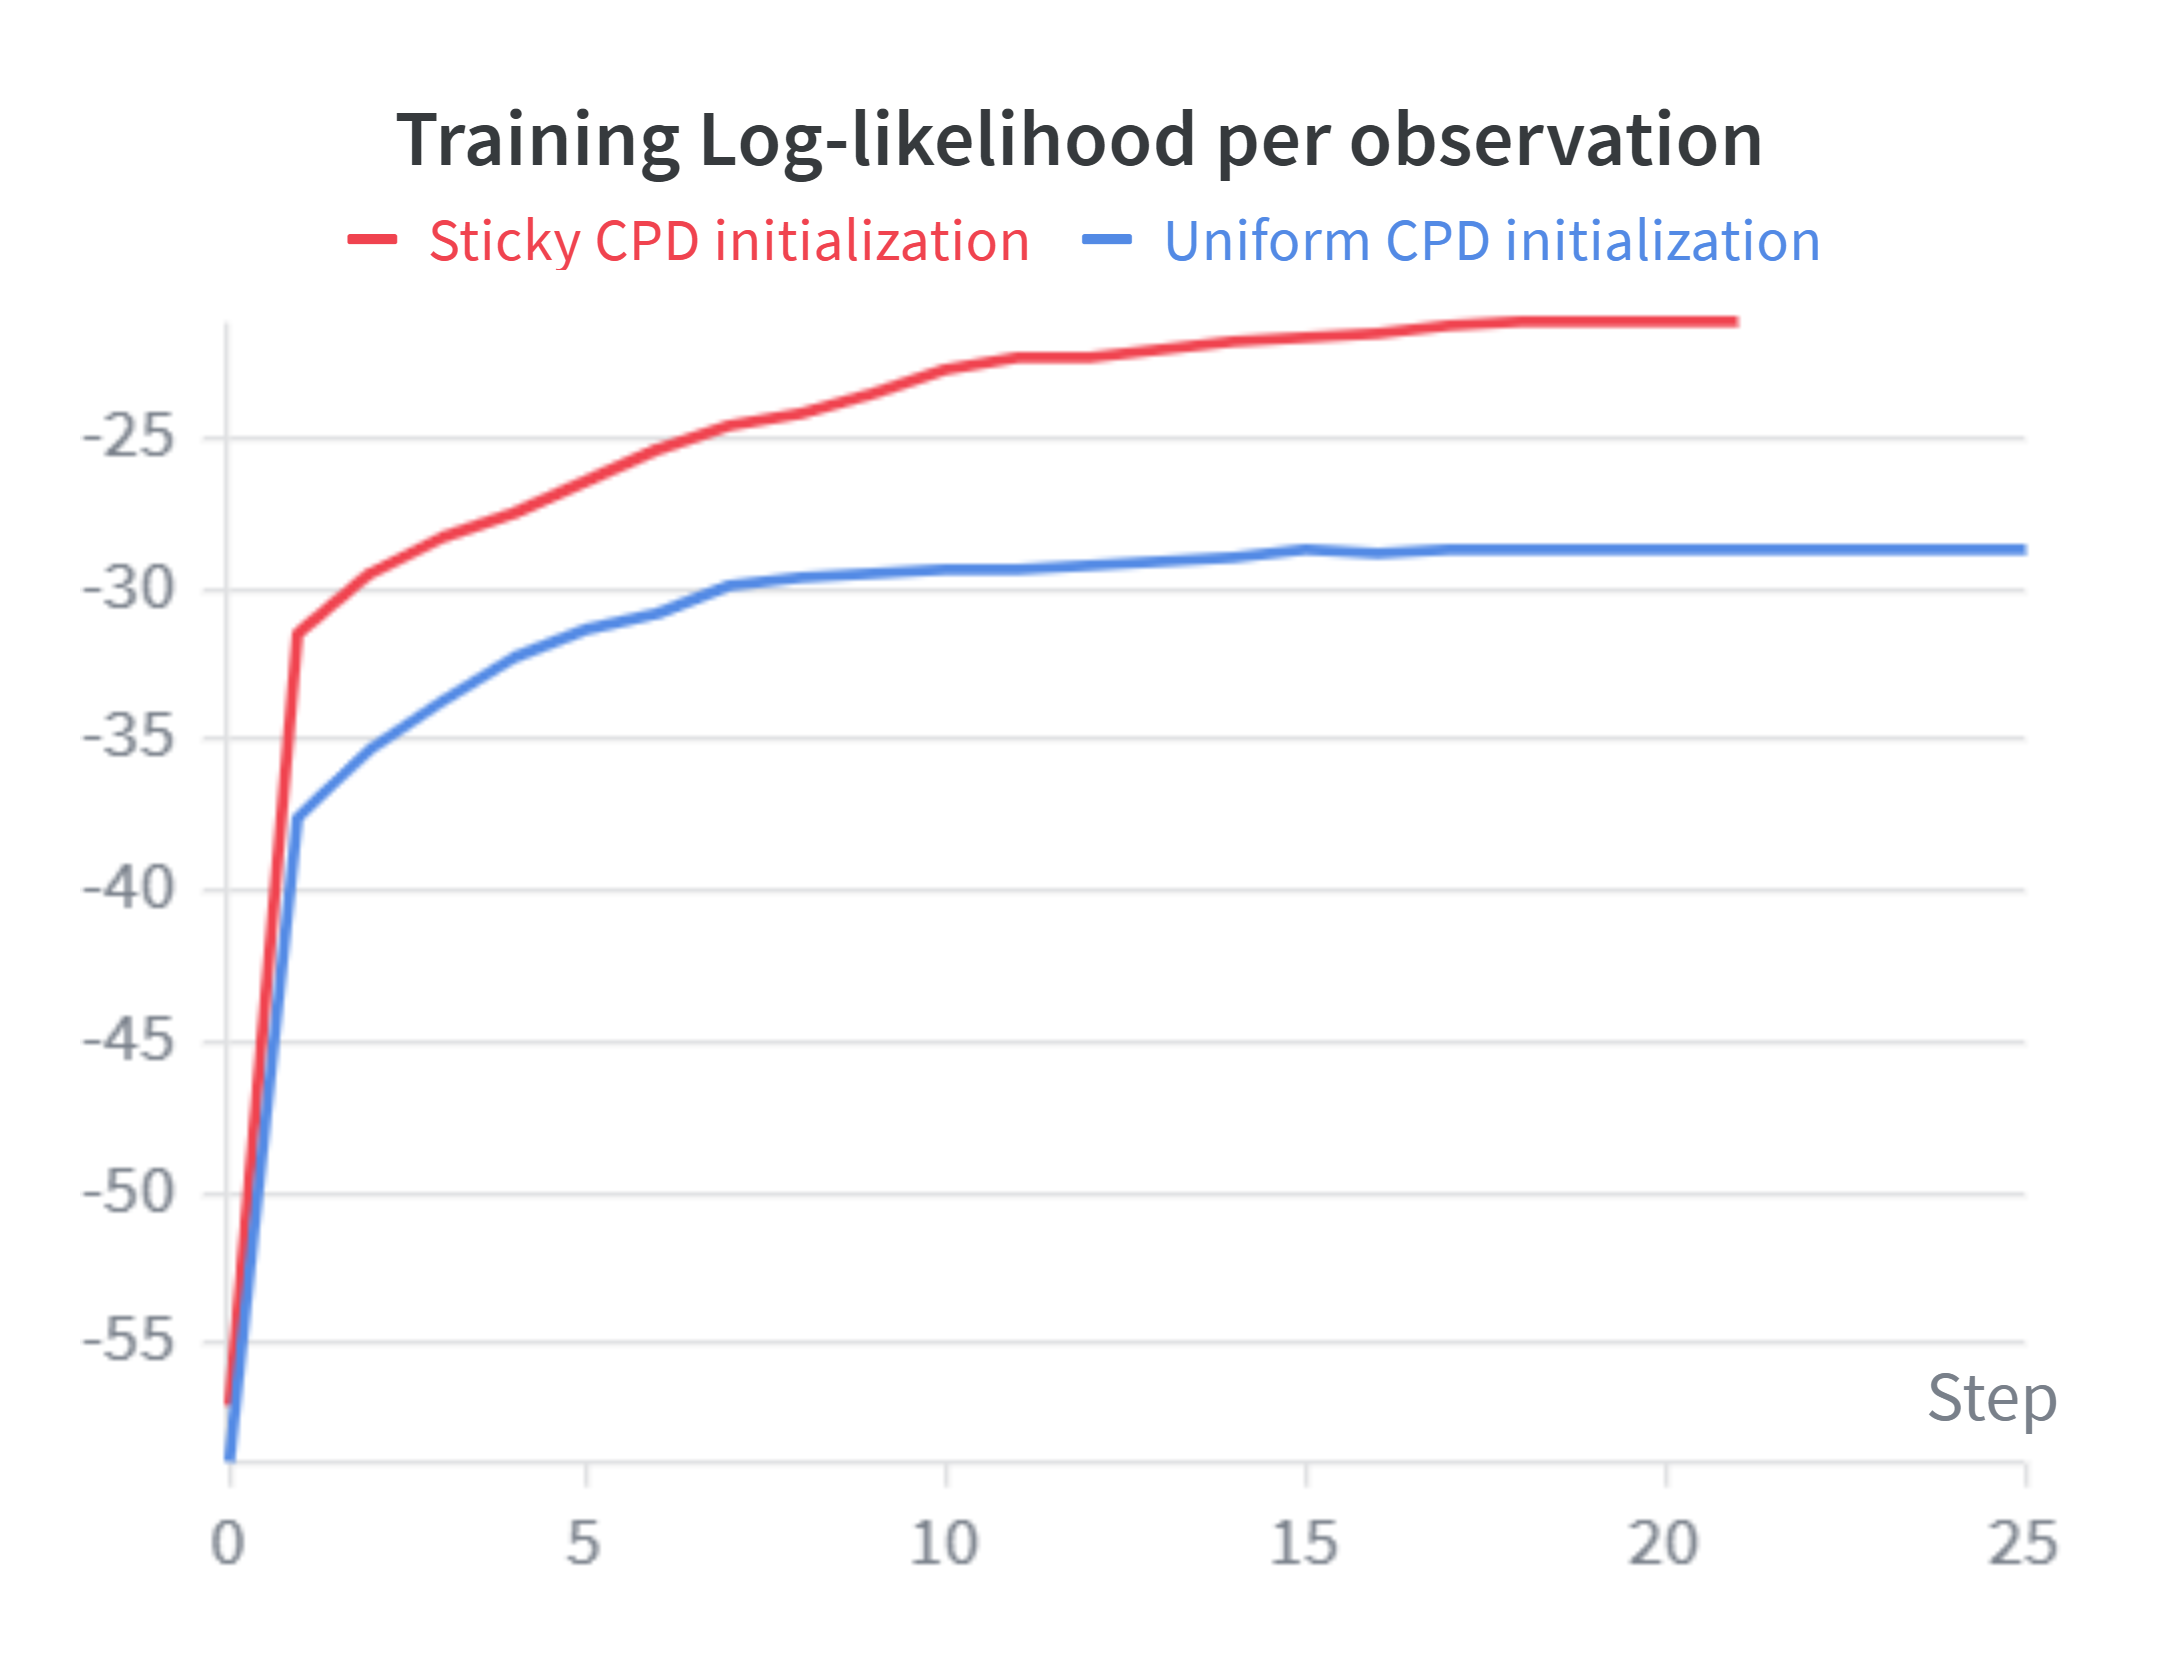
\includegraphics[width=\textwidth]{images/cpd_choice_training.png}
        \label{fig:cpd_init_training}
    \end{subfigure}
    \hfill
    \begin{subfigure}[b]{0.48\textwidth}
        \centering
        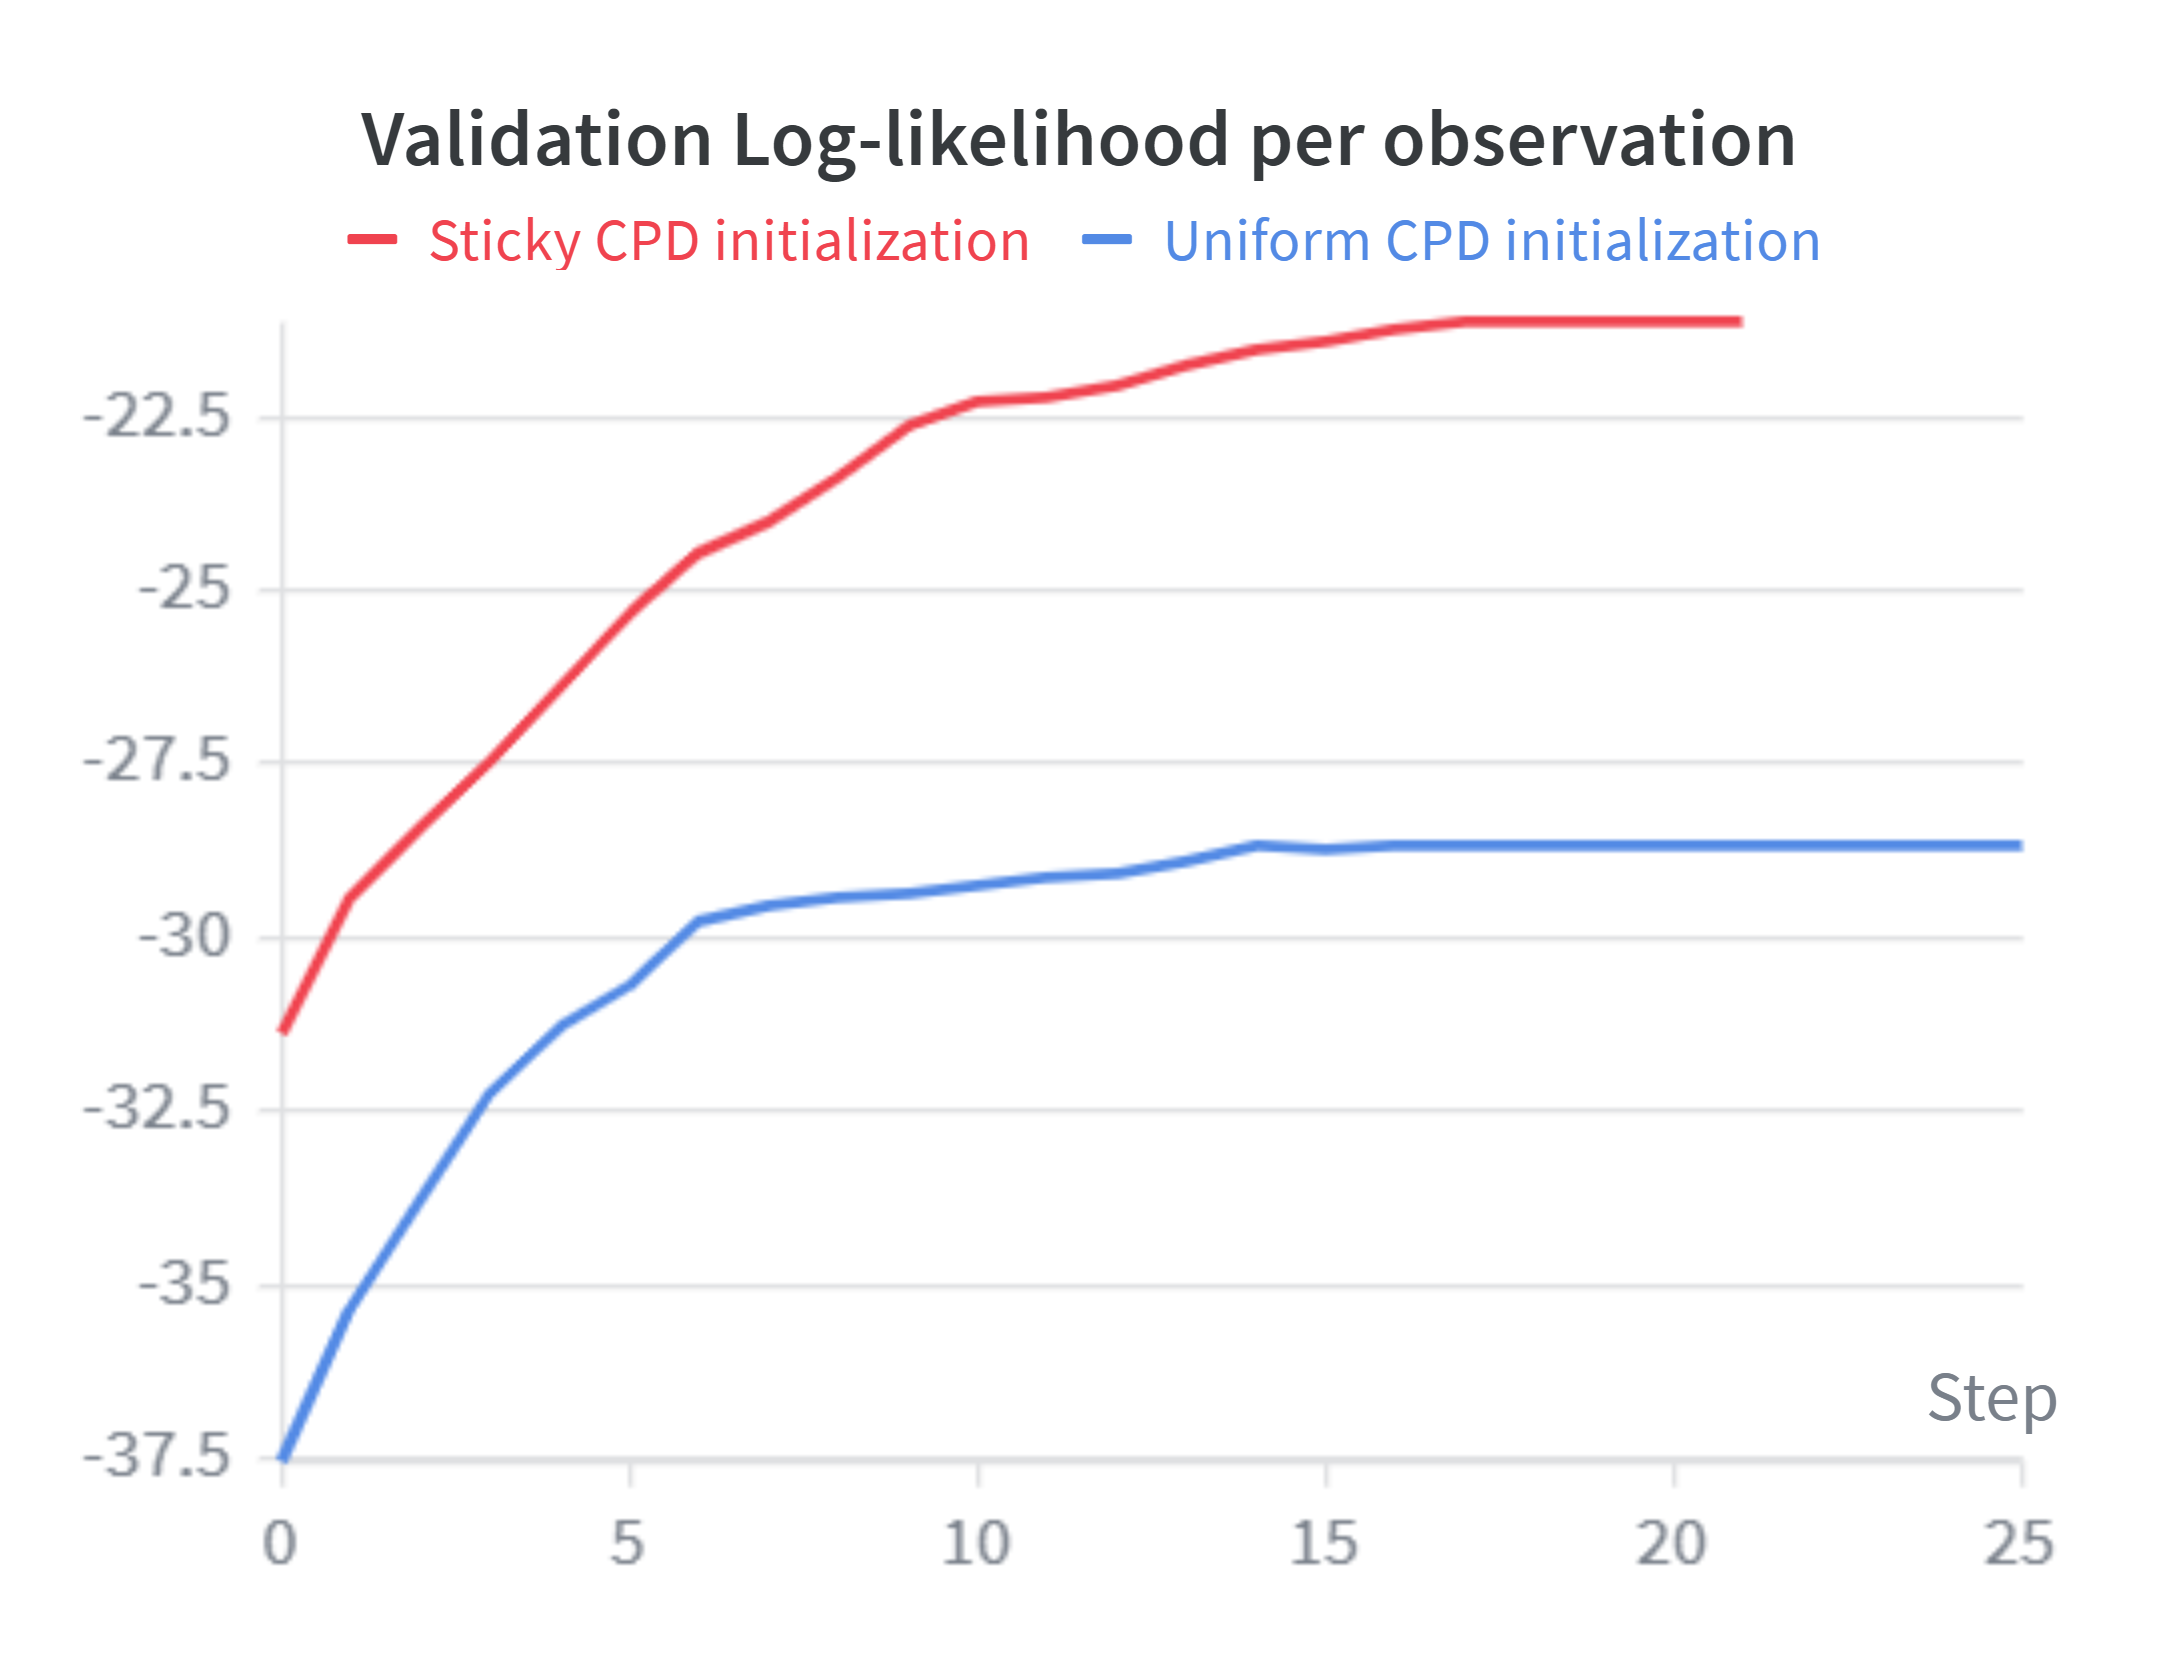
\includegraphics[width=\textwidth]{images/cpd_choice_validation.png}
        \label{fig:cpd_init_validation}
    \end{subfigure}
    \caption[Comparison of sticky vs.\ uniform CPD initialization]{Comparison of sticky vs.\ uniform CPD initialization for the hierarchical emission model (lc-none, Bernoulli enabled, uniform initial distribution).}
    \label{fig:cpd_init_comparison}
\end{figure}

\subsection{Compared Configurations}
The first comparison factor is the emission model.  
This factor examines whether a more structured but constrained emission model is preferable to a more flexible joint observation model. 

\par The second factor is the treatment of the initial latent-state distribution. 
The two variants, are defined in \autoref{subsec:em_training}. Here they are compared only in terms of their effect on overall predictive behavior.

\par The third factor is lane-change weighting. 
Three settings, as defined in \autoref{tab:lc_weight_modes}, are compared. 

\par The fourth factor is the inclusion of Bernoulli likelihood terms for the binary part of the observation vector. 
This makes it possible to assess whether explicit modeling of the binary components improves latent-state separation and prediction quality 
enough to justify the additional complexity.

\subsection{Overview of S2A4 Comparison Results}
\par Table~\ref{tab:s2a4_overview} summarizes the results of the 24 configurations in the main S2A4 study. Lower values of \ac{NLL} and \ac{BIC} indicate better performance. 
Here, $N_{\mathrm{eff}}^{\mathrm{joint}}$ denotes the effective number of jointly used latent states, and $p_{\max}^{\mathrm{joint}}$ denotes 
the maximum joint-state occupancy. BIC values are reported in millions.
Rather than discussing each run separately, the following subsections analyze the results by grouping them according to the design factor under study.
\begin{table}[htbp]
\centering
\caption{Overview of the 24 compared configurations in the main S2A4 study.}
\label{tab:s2a4_overview}
\resizebox{\textwidth}{!}{%
\begin{tabular}{c l c c c c c c c c}
\toprule
Exp. & Emission & Init. dist. & LC mode & Bern. & NLL & BIC [M] & $k$ & $N_{\mathrm{eff}}^{\mathrm{joint}}$ & $p_{\max}^{\mathrm{joint}}$ \\
\midrule
1  & PoE          & uniform & none & off & 28.05 & 66.66 & 518 & 6.37 & 0.26 \\
2  & PoE          & uniform & none & on  & 28.16 & 66.71 & 530 & 6.36 & 0.26 \\
3  & PoE          & uniform & A    & off & 28.08 & 128.76 & 518 & 6.37 & 0.26 \\
4  & PoE          & uniform & A    & on  & 28.13 & 131.95 & 530 & 6.36 & 0.26 \\
5  & PoE          & uniform & B    & off & 30.20 & 71.38 & 518 & 4.89 & 0.29 \\
6  & PoE          & uniform & B    & on  & 30.18 & 71.35 & 530 & 4.88 & 0.29 \\
7  & PoE          & learned & none & off & 28.02 & 59.47 & 525 & 6.36 & 0.26 \\
8  & PoE          & learned & none & on  & 28.20 & 65.08 & 537 & 6.36 & 0.26 \\
9  & PoE          & learned & A    & off & 28.03 & 115.18 & 525 & 6.36 & 0.26 \\
10 & PoE          & learned & A    & on  & 28.17 & 129.12 & 537 & 6.36 & 0.26 \\
11 & PoE          & learned & B    & off & 30.22 & 67.18 & 525 & 4.89 & 0.29 \\
12 & PoE          & learned & B    & on  & 30.16 & 70.85 & 537 & 4.88 & 0.29 \\
13 & Hierarchical & uniform & none & off & 21.93 & 53.28 & 682 & 6.95 & 0.19 \\
14 & Hierarchical & uniform & none & on  & 20.97 & 50.82 & 698 & 6.82 & 0.22 \\
15 & Hierarchical & uniform & A    & off & 20.92 & 99.33 & 682 & 6.84 & 0.22 \\
16 & Hierarchical & uniform & A    & on  & 21.98 & 104.35 & 698 & 6.95 & 0.19 \\
17 & Hierarchical & uniform & B    & off & 22.81 & 55.43 & 682 & 6.13 & 0.22 \\
18 & Hierarchical & uniform & B    & on  & 22.86 & 55.50 & 698 & 6.13 & 0.22 \\
19 & Hierarchical & learned & none & off & 21.92 & 53.26 & 689 & 6.95 & 0.19 \\
20 & Hierarchical & learned & none & on  & 21.99 & 53.39 & 705 & 6.94 & 0.19 \\
21 & Hierarchical & learned & A    & off & 20.92 & 99.29 & 689 & 6.83 & 0.22 \\
22 & Hierarchical & learned & A    & on  & 21.97 & 104.33 & 705 & 6.94 & 0.19 \\
23 & Hierarchical & learned & B    & off & 22.79 & 55.41 & 689 & 6.14 & 0.22 \\
24 & Hierarchical & learned & B    & on  & 22.83 & 55.46 & 705 & 6.13 & 0.22 \\
\bottomrule
\end{tabular}%
}
\end{table}

Across the 24 compared configurations, the hierarchical models outperform the PoE models in \ac{NLL}. 
Within the hierarchical family, lc-none gives the most reliable results, while lc-B consistently over-constrains the latent-state dynamics. 

\subsection{PoE versus Hierarchical Emissions}
To isolate the effect of the emission-model formulation, each \ac{PoE} configuration can be compared with its hierarchical counterpart under the same initial-distribution setting, 
lane-change weighting mode, and Bernoulli setting. 
Across all 12 matched pairs in Table~\ref{tab:s2a4_overview}, the hierarchical emission model achieves lower \ac{NLL} than the corresponding \ac{PoE} model. 
The same trend is reflected in \ac{BIC}, despite the larger number of parameters in the hierarchical model.

\par This indicates that the additional flexibility of the hierarchical emission model is beneficial for the window-based highway-driving observations considered here, 
whereas the more structured \ac{PoE} formulation appears too restrictive.

\par The posterior diagnostics also favor the hierarchical family.  
Its effective number of jointly used latent states is generally higher, while the maximum occupancy of a single joint state is lower than in the corresponding \ac{PoE} runs. 
This suggests a more balanced use of the latent-state space, whereas the \ac{PoE} models tend to concentrate more probability mass on fewer joint states.

\par Based on these results, the hierarchical emission model is retained as the stronger observation model.

\subsection{Effect of Bernoulli Likelihood Terms}
To examine the effect of explicitly modeling the binary components of the observation vector, each configuration with Bernoulli likelihoods disabled is compared with the 
corresponding configuration in which they are enabled, while keeping the emission model, initial-distribution setting, and lane-change weighting mode fixed. 
The effect is not uniform across the experiment grid.

\par For the \ac{PoE} models, enabling the Bernoulli terms does not produce a consistent improvement. 
In most matched pairs, \ac{NLL} becomes slightly worse, while the parameter count increases from $k=518$ to $k=530$ or from $k=525$ to $k=537$. 
As a result, the \ac{BIC} is usually unchanged. 
Only very small gains appear in the lc-B setting, and these are too marginal to indicate a meaningful advantage.

\par For the hierarchical models, the picture is mixed. 
In the principled lc-none setting with a fixed uniform initial distribution, enabling Bernoulli terms gives a clear benefit: the \ac{NLL} improves from 21.93 in Exp.~13 to 20.97 
in Exp.~14, and \ac{BIC} improves from 53.28\,M to 50.82\,M despite the higher parameter count. 
This is the only case in which the binary likelihood terms clearly improve both measures.

\par However, this benefit does not generalize across the full hierarchical family.  
With learned initial distributions in the lc-none setting, the Bernoulli version is slightly worse than its non-Bernoulli counterpart (Exp.~20 versus Exp.~19). 
In the lc-A and lc-B settings, enabling Bernoulli terms is again neutral or negative, with a substantial degradation in the lc-A case. 
This indicates that the usefulness of the binary likelihood terms depends on the surrounding modeling choices rather than providing a uniform improvement by themselves.

\subsection{Effect of Learning the Initial Distribution}
To evaluate the role of the initial latent-state distribution, each configuration with a fixed uniform initial distribution is compared with the corresponding configuration 
in which the initial distribution is learned, while the emission model, lane-change weighting mode, and Bernoulli setting remain unchanged. 
Overall, learning the initial distribution has only a limited effect on the final results.

\par In the \ac{PoE} family, learning the initial distribution sometimes improves the likelihood-based scores, especially in the lc-none setting with Bernoulli terms disabled, 
where the \ac{NLL} decreases slightly from 28.05 in Exp.~1 to 28.02 in Exp.~7 and the \ac{BIC} improves more clearly from 66.66\,M to 59.47\,M. 
A similar pattern is visible for the lc-A setting without Bernoulli terms, where Exp.~9 performs slightly better than Exp.~3. 
However, these gains are not stable across all \ac{PoE} runs, since some Bernoulli-enabled settings become slightly worse.

\par In the hierarchical family, the effect is even smaller. 
Across most matched pairs, the results with learned and fixed initial distributions are nearly identical. 
For example, in the lc-none setting with Bernoulli terms disabled, Exp.~19 and Exp.~13 differ only marginally in both \ac{NLL} and \ac{BIC}. 
When Bernoulli terms are enabled, the learned-initial-distribution variant is slightly worse than the fixed one in the same lc-none setting (Exp.~20 versus Exp.~14). 
The same weak pattern appears in the weighted settings, where the differences remain small compared with the stronger effects of the emission model and lane-change weighting.

\par These results suggest that the long-run behavior is governed much more by the transition and emission structure than by the precise 
choice of the initial latent belief. 
Since the observation sequences are long enough for filtering to move away from the initial distribution after only a few steps, changes in the initialization affect mainly 
the early part of each sequence and do not strongly alter the overall fit. 
For this reason, learning the initial distribution is not treated as a decisive factor in the final model choice. 
It can provide minor gains in some \ac{PoE} runs, but within the better-performing hierarchical family it does not yield a consistent improvement. 
Accordingly, the final selection is based mainly on the emission model and the lane-change weighting setting rather than on this factor.

\subsection{Effect of Lane-Change Weighting}
For each emission model, initial-distribution setting, and Bernoulli setting, three variants are compared: the unweighted lc-none baseline, lc-A, and lc-B.  
This factor is especially relevant because lane-change events are sparse in the selected subset, which naturally motivates giving more emphasis to these rare but important maneuvers.

\par The clearest pattern is that lc-B consistently degrades the results. 
Across both emission families and across both initial-distribution settings, lc-B yields noticeably worse \ac{NLL} values than lc-none. 
The posterior diagnostics also become less favorable. The effective number of jointly used latent states decreases, while the maximum occupancy of a single joint state increases. 
For example, in the \ac{PoE} runs, $N_{\mathrm{eff}}^{\mathrm{joint}}$ falls from about 6.36 in the lc-none setting to about 4.88 in lc-B, 
while $p_{\max}^{\mathrm{joint}}$ rises from 0.26 to 0.29. 
A similar, though less pronounced, reduction in effective joint-state usage appears in the hierarchical family. 
This indicates that lc-B pushes the model toward a less balanced use of the latent-state space and therefore over-constrains the learned dynamics.

\par The lc-A setting is more ambiguous. 
In some hierarchical runs, especially without Bernoulli terms, lc-A gives slightly lower \ac{NLL} values than lc-none. 
For instance, Exp.~15 and Exp.~21 achieve lower \ac{NLL} values than their lc-none counterparts Exp.~13 and Exp.~19. 
However, this effect is not stable across the full comparison grid. 
When Bernoulli terms are enabled, the advantage disappears or becomes very small, and in the \ac{PoE} family lc-A does not provide a convincing overall benefit.  
Moreover, the \ac{BIC} values under lc-A are consistently much less favorable than in the corresponding lc-none runs.

\par Although lc-A can sometimes improve the likelihood-based score, these gains are not treated as decisive because lc-A modifies inference heuristically rather 
than preserving the same probabilistic interpretation as the unweighted model. 
A lower score under lc-A therefore does not carry the same weight as an improvement obtained under the standard lc-none formulation.

\par Taken together, these findings support lc-none as the most principled and reliable choice.  
It avoids the clear degradation seen under lc-B and does not rely on the heuristic bias introduced by lc-A. 

\subsection{Summary of Selected Core Model}
Based on the main S2A4 comparison, Exp.~14 is selected as the core model for the remainder of this chapter. 
This model uses hierarchical emissions, sticky \acp{CPD} initialization, a fixed uniform initial latent-state distribution, no lane-change weighting (lc-none), 
and Bernoulli likelihood terms enabled. 
It is selected because it provides the strongest overall combination of fit quality and balanced latent-state usage in the unweighted setting.

\par It achieves an \ac{NLL} of 20.97 and a \ac{BIC} of 50.82\,M, while showing balanced use of the latent space with $N_{\mathrm{eff}}^{\mathrm{joint}} = 6.82$ 
and $p_{\max}^{\mathrm{joint}} = 0.22$. 
On the held-out test set, the model uses both style states effectively, with $k_{\mathrm{eff}}^{\mathrm{style}} \approx 2.00$, and also makes substantial 
use of the action latent space, with $k_{\mathrm{eff}}^{\mathrm{action}} \approx 3.72$.

\par The learned transition structure is consistent with the intended interpretation of the model, 
with persistent style states and mostly persistent action states. 
This supports the factorization in which style captures the broader behavioral regime while action captures shorter-term maneuver dynamics 
within that regime.

\begin{figure}[htbp]
    \centering
    \begin{subfigure}[b]{0.32\textwidth}
        \centering
        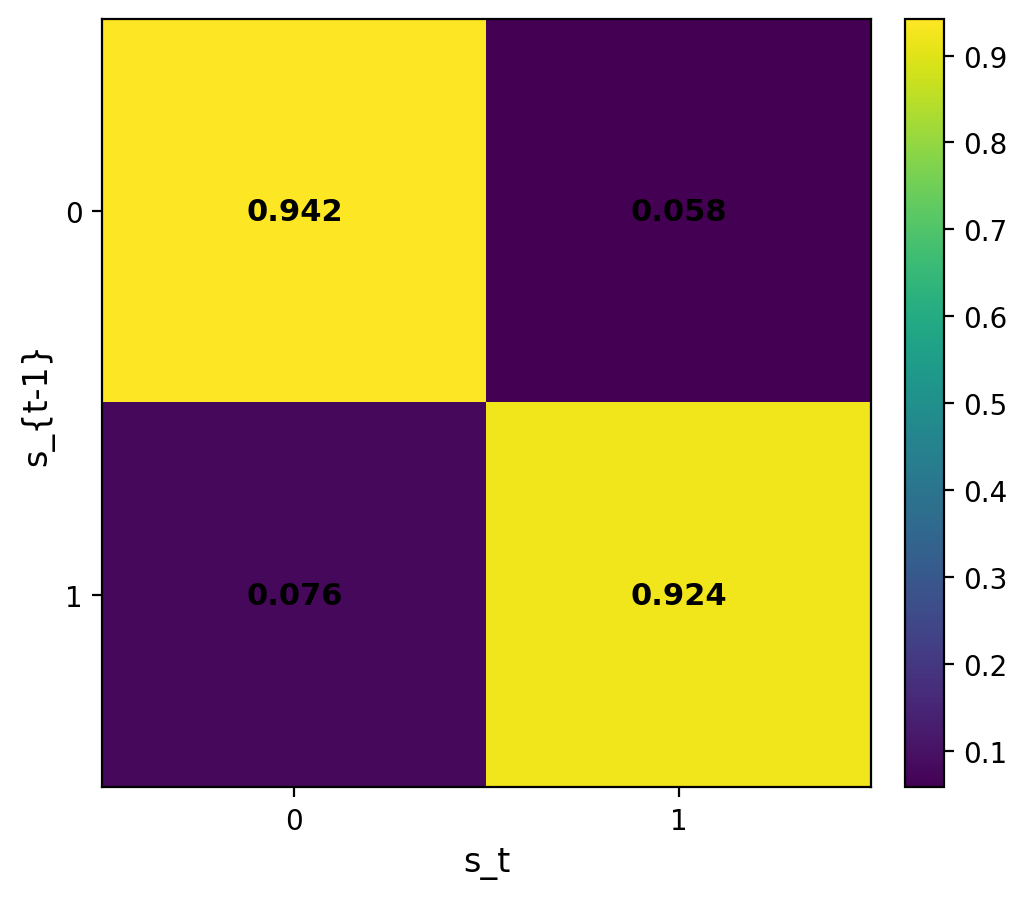
\includegraphics[width=\textwidth]{images/A_s.png}
        \caption{Style transition matrix}
        \label{fig:selected_style_transition}
    \end{subfigure}
    \hfill
    \begin{subfigure}[b]{0.32\textwidth}
        \centering
        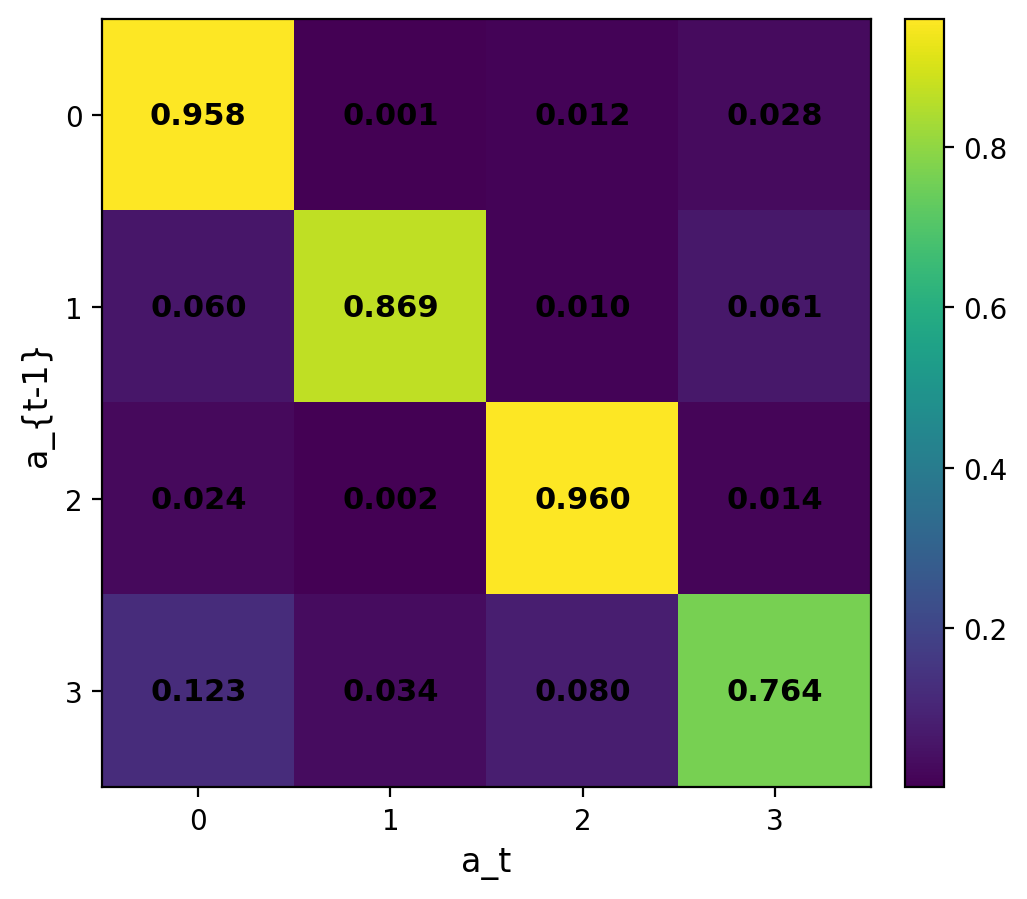
\includegraphics[width=\textwidth]{images/A_a_style_0.png}
        \caption{Action transitions for $s=0$}
        \label{fig:selected_action_transition_s0}
    \end{subfigure}
    \hfill
    \begin{subfigure}[b]{0.32\textwidth}
        \centering
        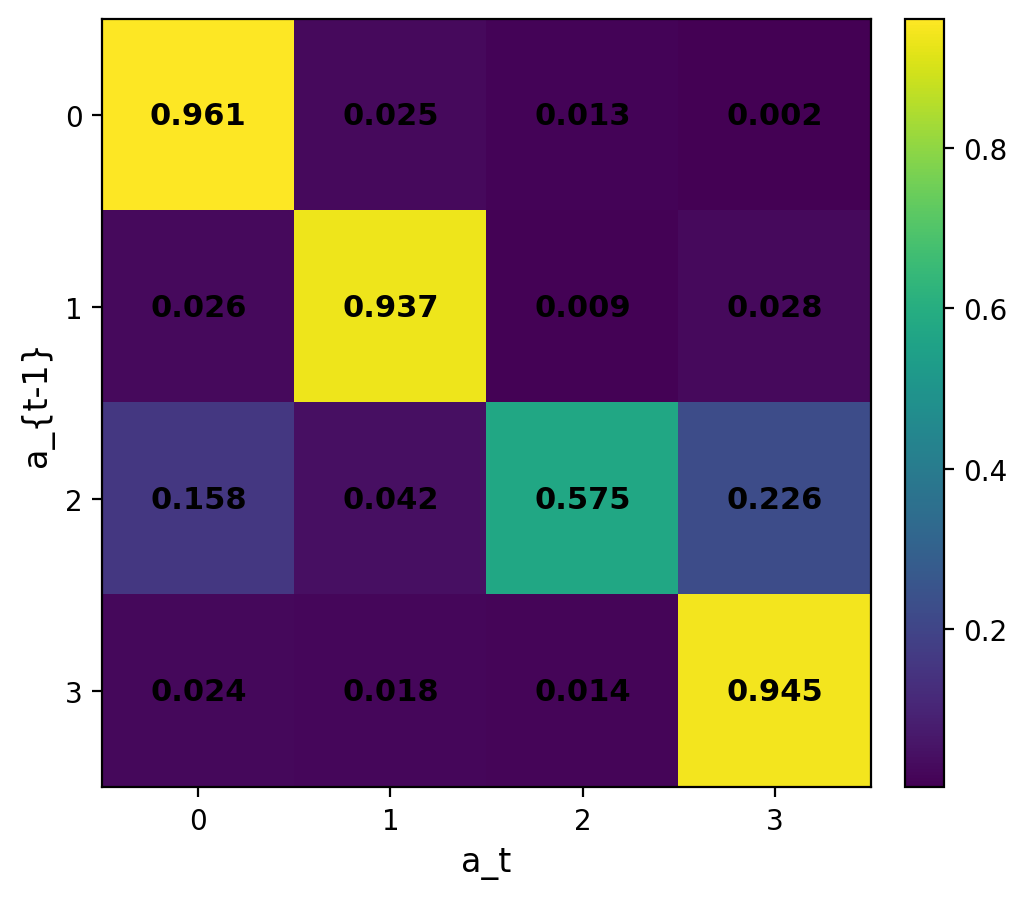
\includegraphics[width=\textwidth]{images/A_a_style_1.png}
        \caption{Action transitions for $s=1$}
        \label{fig:selected_action_transition_s1}
    \end{subfigure}
    \caption[Learned transition structure of the selected core model]{Learned transition structure of the selected core model (Exp.~14).}
    \label{fig:selected_core_model_transitions}
\end{figure}
Figure~\ref{fig:selected_core_model_transitions} further illustrates the learned transition structure of the selected model. 

\subsection{Semantic Interpretation of the Learned Latent States}
\label{subsec:semantic_interpretation_selected_model}

Following the procedure described in \autoref{sec:semantic_interpretation_latent_states}, the latent states of the selected model  
are assigned semantic labels by examining posterior-weighted feature profiles and applying rule-based heuristics. 
This step is necessary because the \ac{DBN} is trained unsupervised, so the learned states do not initially correspond to named driver behaviors.

\par For the S2A4 hierarchical model, the two style states capture the following regimes:
\begin{itemize}
    \item \textbf{Style $s_0$ (low-interaction):} Motion is relatively smooth and less constrained by surrounding traffic.
    \item \textbf{Style $s_1$ (high-interaction):} Driver behavior is more strongly influenced by nearby vehicles, gap availability, and tactical traffic constraints.
\end{itemize}

Within each style, the four action states represent maneuvers along the following interpretations:
\begin{itemize}
    \item \textbf{$(s_0,a_0)$ -- Free flow:} Unconstrained motion with little or no leader influence, typically at higher speed and with small speed corrections.
    \item \textbf{$(s_0,a_1)$ -- Mild brake:} Sustained but not strongly tactical deceleration while following another vehicle.
    \item \textbf{$(s_0,a_2)$ -- Constrained acceleration:} Acceleration present, but not unconstrained, since surrounding traffic still limits the maneuver.
    \item \textbf{$(s_0,a_3)$ -- Stable following:} Relatively steady car-following with mild control effort and limited speed change.
    \item \textbf{$(s_1,a_0)$ -- Strong acceleration:} Acceleration-dominant behavior in a tactical setting, often with a nearby leader still present.
    \item \textbf{$(s_1,a_1)$ -- Lane change:} Clear lateral motion and associated speed adjustment.
    \item \textbf{$(s_1,a_2)$ -- Constrained following:} Following behavior with tighter interaction, lower speed, or more frequent corrective adjustments than stable following.
    \item \textbf{$(s_1,a_3)$ -- Tactical brake:} Sustained braking under stronger interaction constraints.
\end{itemize}



\subsection{Predictive Performance of the Selected Model}
Using the semantic interpretation defined in \autoref{subsec:semantic_interpretation_selected_model}, the predictive performance of the 
selected model is now evaluated in the causal online setting. 
The reference labeling, warmup handling, and causal prediction protocol follow \autoref{sec:inference_evaluation}.

\subsubsection{Exact One-Step Prediction Performance}
\begin{figure}[H]
    \centering
    
\includegraphics[width=0.96\textwidth]{images/confusion_matrix.png}
    \caption[Confusion matrix for exact one-step prediction]{Confusion matrix for exact one-step joint-state prediction on the test set. Rows denote reference labels and columns denote predicted labels.}
    \label{fig:exact_one_step_confusion_matrix}
\end{figure}

\begin{figure}[H]
    \centering
    \begin{subfigure}[b]{0.75\textwidth}
        \centering
        
\includegraphics[width=\textwidth]{images/confusion_matrix_row_normalized.png}
        \caption{Recall view}
        \label{fig:exact_one_step_confusion_row_norm}
    \end{subfigure}
    \hfill
    \begin{subfigure}[b]{0.75\textwidth}
        \centering
        
\includegraphics[width=\textwidth]{images/confusion_matrix_column_normalized.png}
        \caption{Precision view}
        \label{fig:exact_one_step_confusion_col_norm}
    \end{subfigure}
    \caption[Row and column-normalized confusion matrices]{Row and column-normalized confusion matrices.}
    \label{fig:exact_one_step_confusion_normalized}
\end{figure}

Under the strict joint-state evaluation, the selected model achieves an exact next-step accuracy of 46.37\%.
The macro precision, recall, and F1-score are 44.35\%, 48.18\%, and 42.25\%, respectively.
These values indicate that the one-step prediction task is challenging, especially because several maneuver classes are very similar to each other.

\par The confusion matrix in Figure~\ref{fig:exact_one_step_confusion_matrix} shows that the model identifies clearly distinguishable maneuvers such as 
free-flow driving, lane changes, strong acceleration, and tactical braking relatively well. However,
semantically closer longitudinal behaviors such as mild braking, stable following, constrained acceleration, and constrained following remain strongly overlapped.

\par The row-normalized confusion matrix in Figure~\ref{fig:exact_one_step_confusion_row_norm} shows how well each true class is recovered.
Free flow is predicted well, and tactical braking is also recognized clearly.
Strong acceleration is identified reasonably well.
The main errors occur between semantically similar classes: mild brake is often confused with tactical brake, constrained acceleration with strong acceleration,
and both following classes are distributed across nearby classes.

\par The column-normalized view in Figure~\ref{fig:exact_one_step_confusion_col_norm} leads to a similar conclusion.
It highlights prediction reliability: free-flow and lane-change predictions are comparatively precise, whereas mild-brake, constrained-acceleration, and following-related predictions are less precise
because their predicted columns contain multiple related true classes.

\par The class-wise precision, recall, and F1-score further support this interpretation.

\begin{table}[H]
\centering
\caption{Class-wise precision, recall, and F1-score for exact one-step joint-state prediction.}
\label{tab:classwise_prf_exact}
\begin{tabular}{lccc}
\toprule
Class & Precision [\%] & Recall [\%] & F1 [\%] \\
\midrule
low\_interaction/free\_flow               & 85.01 & 89.64 & 87.26 \\
low\_interaction/mild\_brake              & 3.07  & 24.34 & 5.45  \\
low\_interaction/constrained\_acceleration& 17.68 & 36.74 & 23.87 \\
low\_interaction/stable\_following        & 27.58 & 19.26 & 22.68 \\
high\_interaction/strong\_acceleration    & 56.41 & 60.46 & 58.37 \\
high\_interaction/lane\_change            & 53.40 & 65.50 & 58.83 \\
high\_interaction/constrained\_following  & 51.92 & 6.93  & 12.22 \\
high\_interaction/tactical\_brake         & 59.71 & 82.55 & 69.30 \\
\bottomrule
\end{tabular}
\end{table}

\par The \autoref{tab:classwise_prf_exact} shows that free flow is the most clearly identifiable class, with high precision and recall.
Tactical brake, Strong acceleration and lane change are also recognized moderately well.
In contrast, mild brake performs very poorly, which suggests that weak braking behavior does not form a sufficiently distinct class under the current feature 
representation and semantic mapping.
The two following-related classes are also difficult to separate cleanly.
In particular, constrained\_following has moderate precision but extremely low recall, which means that the model predicts this class only rarely and 
assigns many of its true samples to neighboring classes instead.
Overall, these class-wise metrics confirm that the proposed model captures the broad behavioral structure, 
but still struggles with fine-grained distinctions between semantically similar longitudinal maneuvers.

\begin{figure}[H]
    \centering
    
\includegraphics[width=0.75\textwidth]{images/confusion_matrix_grouped.png}
    \caption[Grouped confusion matrix for exact one-step prediction]{Grouped confusion matrix for exact one-step prediction after merging semantically similar maneuver classes.}
    \label{fig:exact_one_step_confusion_grouped}
\end{figure}

\par Figure~\ref{fig:exact_one_step_confusion_grouped} shows that when similar action classes are grouped together, the results improve clearly.
The exact next-step accuracy increases to 62.39\%.
The grouped precision, recall, and F1-score increase to 65.06\%, 70.88\%, and 63.97\%, respectively.
This means that many wrong predictions are not fully wrong.
In many cases, the model predicts a behavior that is close to the true class.

\FloatBarrier

\subsubsection{Horizon-Based Prediction Performance}
The exact next-step metric is very strict.
A prediction is counted as correct only if the predicted class appears at the very next step.
However, in highway traffic, a prediction can still be useful even if the maneuver happens a little later.
For this reason, the selected model is also evaluated over a 2\,s prediction horizon.
As defined in \autoref{sec:inference_evaluation}, this horizon corresponds to the next five future observations.

\par Without grouping similar actions, the model achieves a hit rate of 55.21\% within the 2\,s horizon.
The mean time-to-hit is 0.54\,s, and the median time-to-hit is 0.40\,s.
This shows that when the model makes a successful forecast, the predicted maneuver usually appears very soon after the prediction.
Figure~\ref{fig:horizon_ungrouped} shows that the cumulative hit-rate curve further supports this interpretation, since the largest gain occurs already at the first future step and the curve 
then rises only gradually over the remaining horizon.
This shows that the model is mainly useful for immediate short-horizon prediction.

\begin{figure}[h]
    \centering
    \begin{subfigure}[b]{0.49\textwidth}
        \centering
        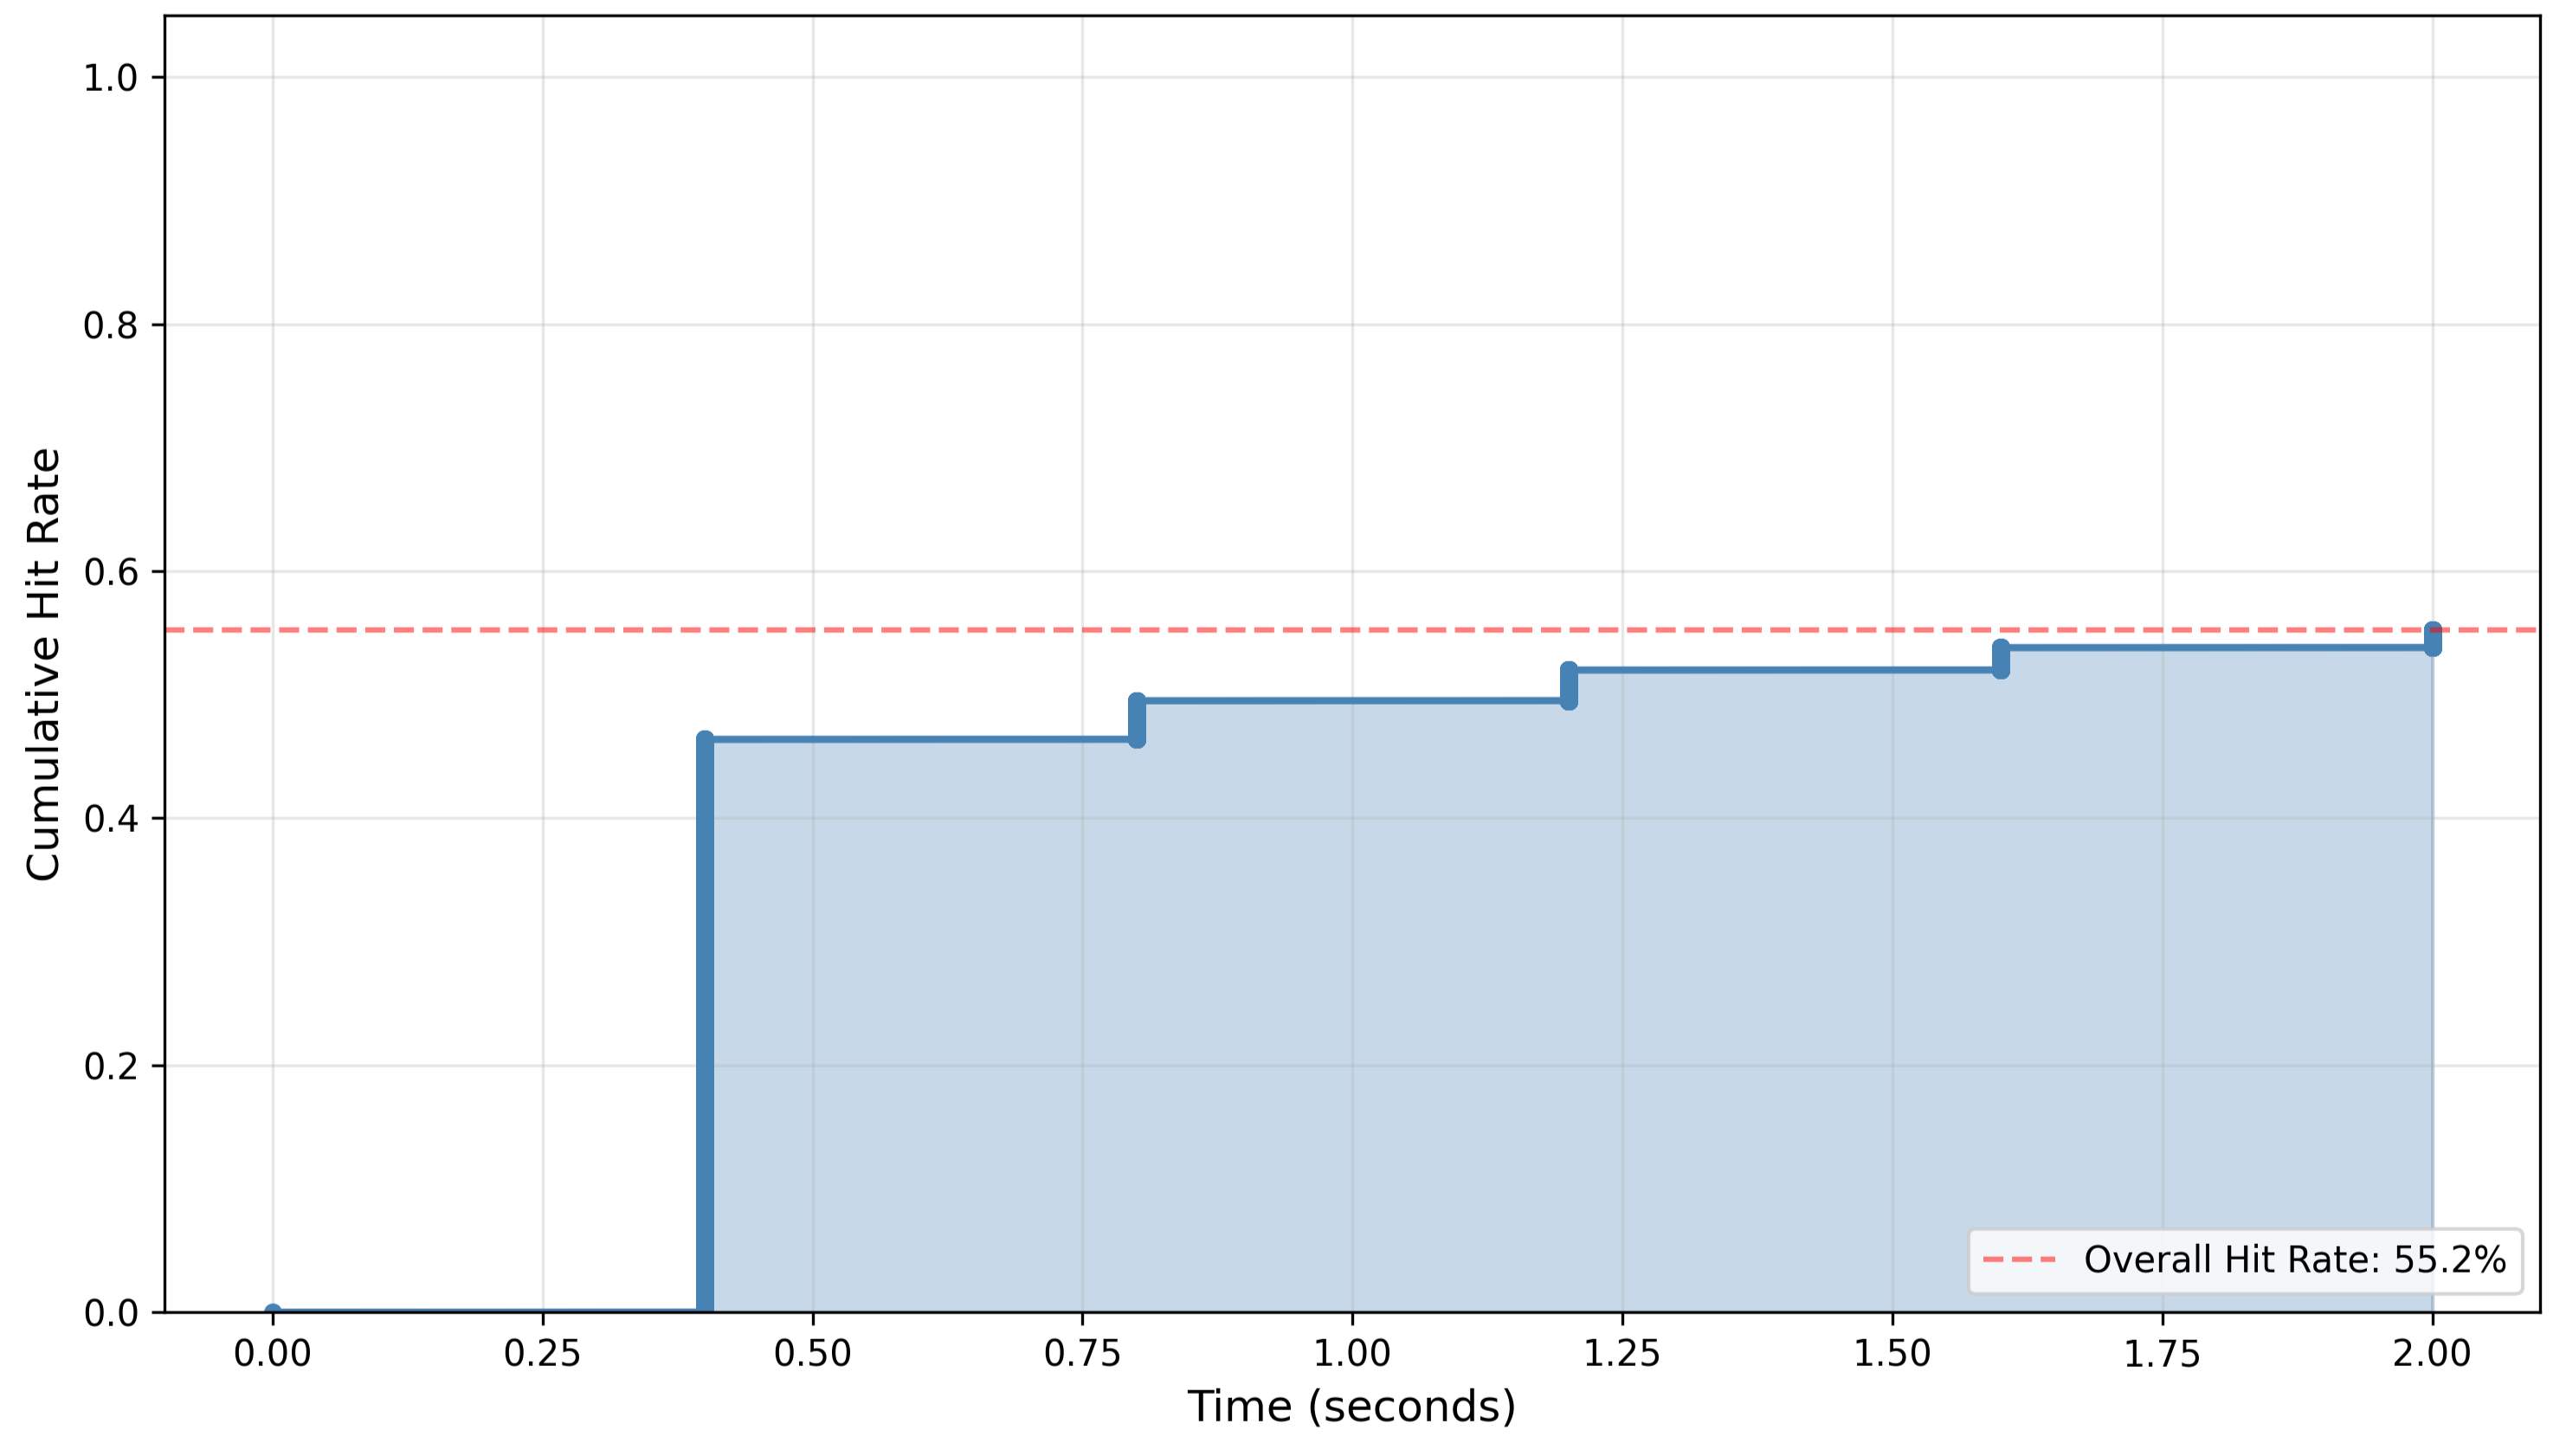
\includegraphics[width=\textwidth]{images/cumulative_hit_rate_ungrouped.png}
        \caption{Cumulative hit rate}
        \label{fig:cumulative_hit_rate_ungrouped}
    \end{subfigure}
    \hfill
    \begin{subfigure}[b]{0.49\textwidth}
        \centering
        
\includegraphics[width=\textwidth]{images/hit_count_summary_ungrouped.png}
        \caption{Hit/miss summary}
        \label{fig:hit_count_summary_ungrouped}
    \end{subfigure}
    \caption[Ungrouped horizon prediction results]{Ungrouped horizon prediction results within the 2\,s forecast horizon.}
    \label{fig:horizon_ungrouped}
\end{figure}

\par When semantically similar actions are grouped, the hit rate increases to 70.20\%.
The mean time-to-hit is 0.50\,s, and the median remains 0.40\,s.
This confirms that many of the misses in the strict ungrouped evaluation are near-misses between related behaviors, especially within the acceleration, 
braking, and following classes.
From an application point of view, this is an encouraging result, since predicting the correct broader maneuver tendency within a short time interval is often 
more important than identifying the exact fine-grained subclass at the very next step. Figure~\ref{fig:horizon_grouped} shows the grouped horizon results.

\begin{figure}[h]
    \centering
    \begin{subfigure}[b]{0.49\textwidth}
        \centering
        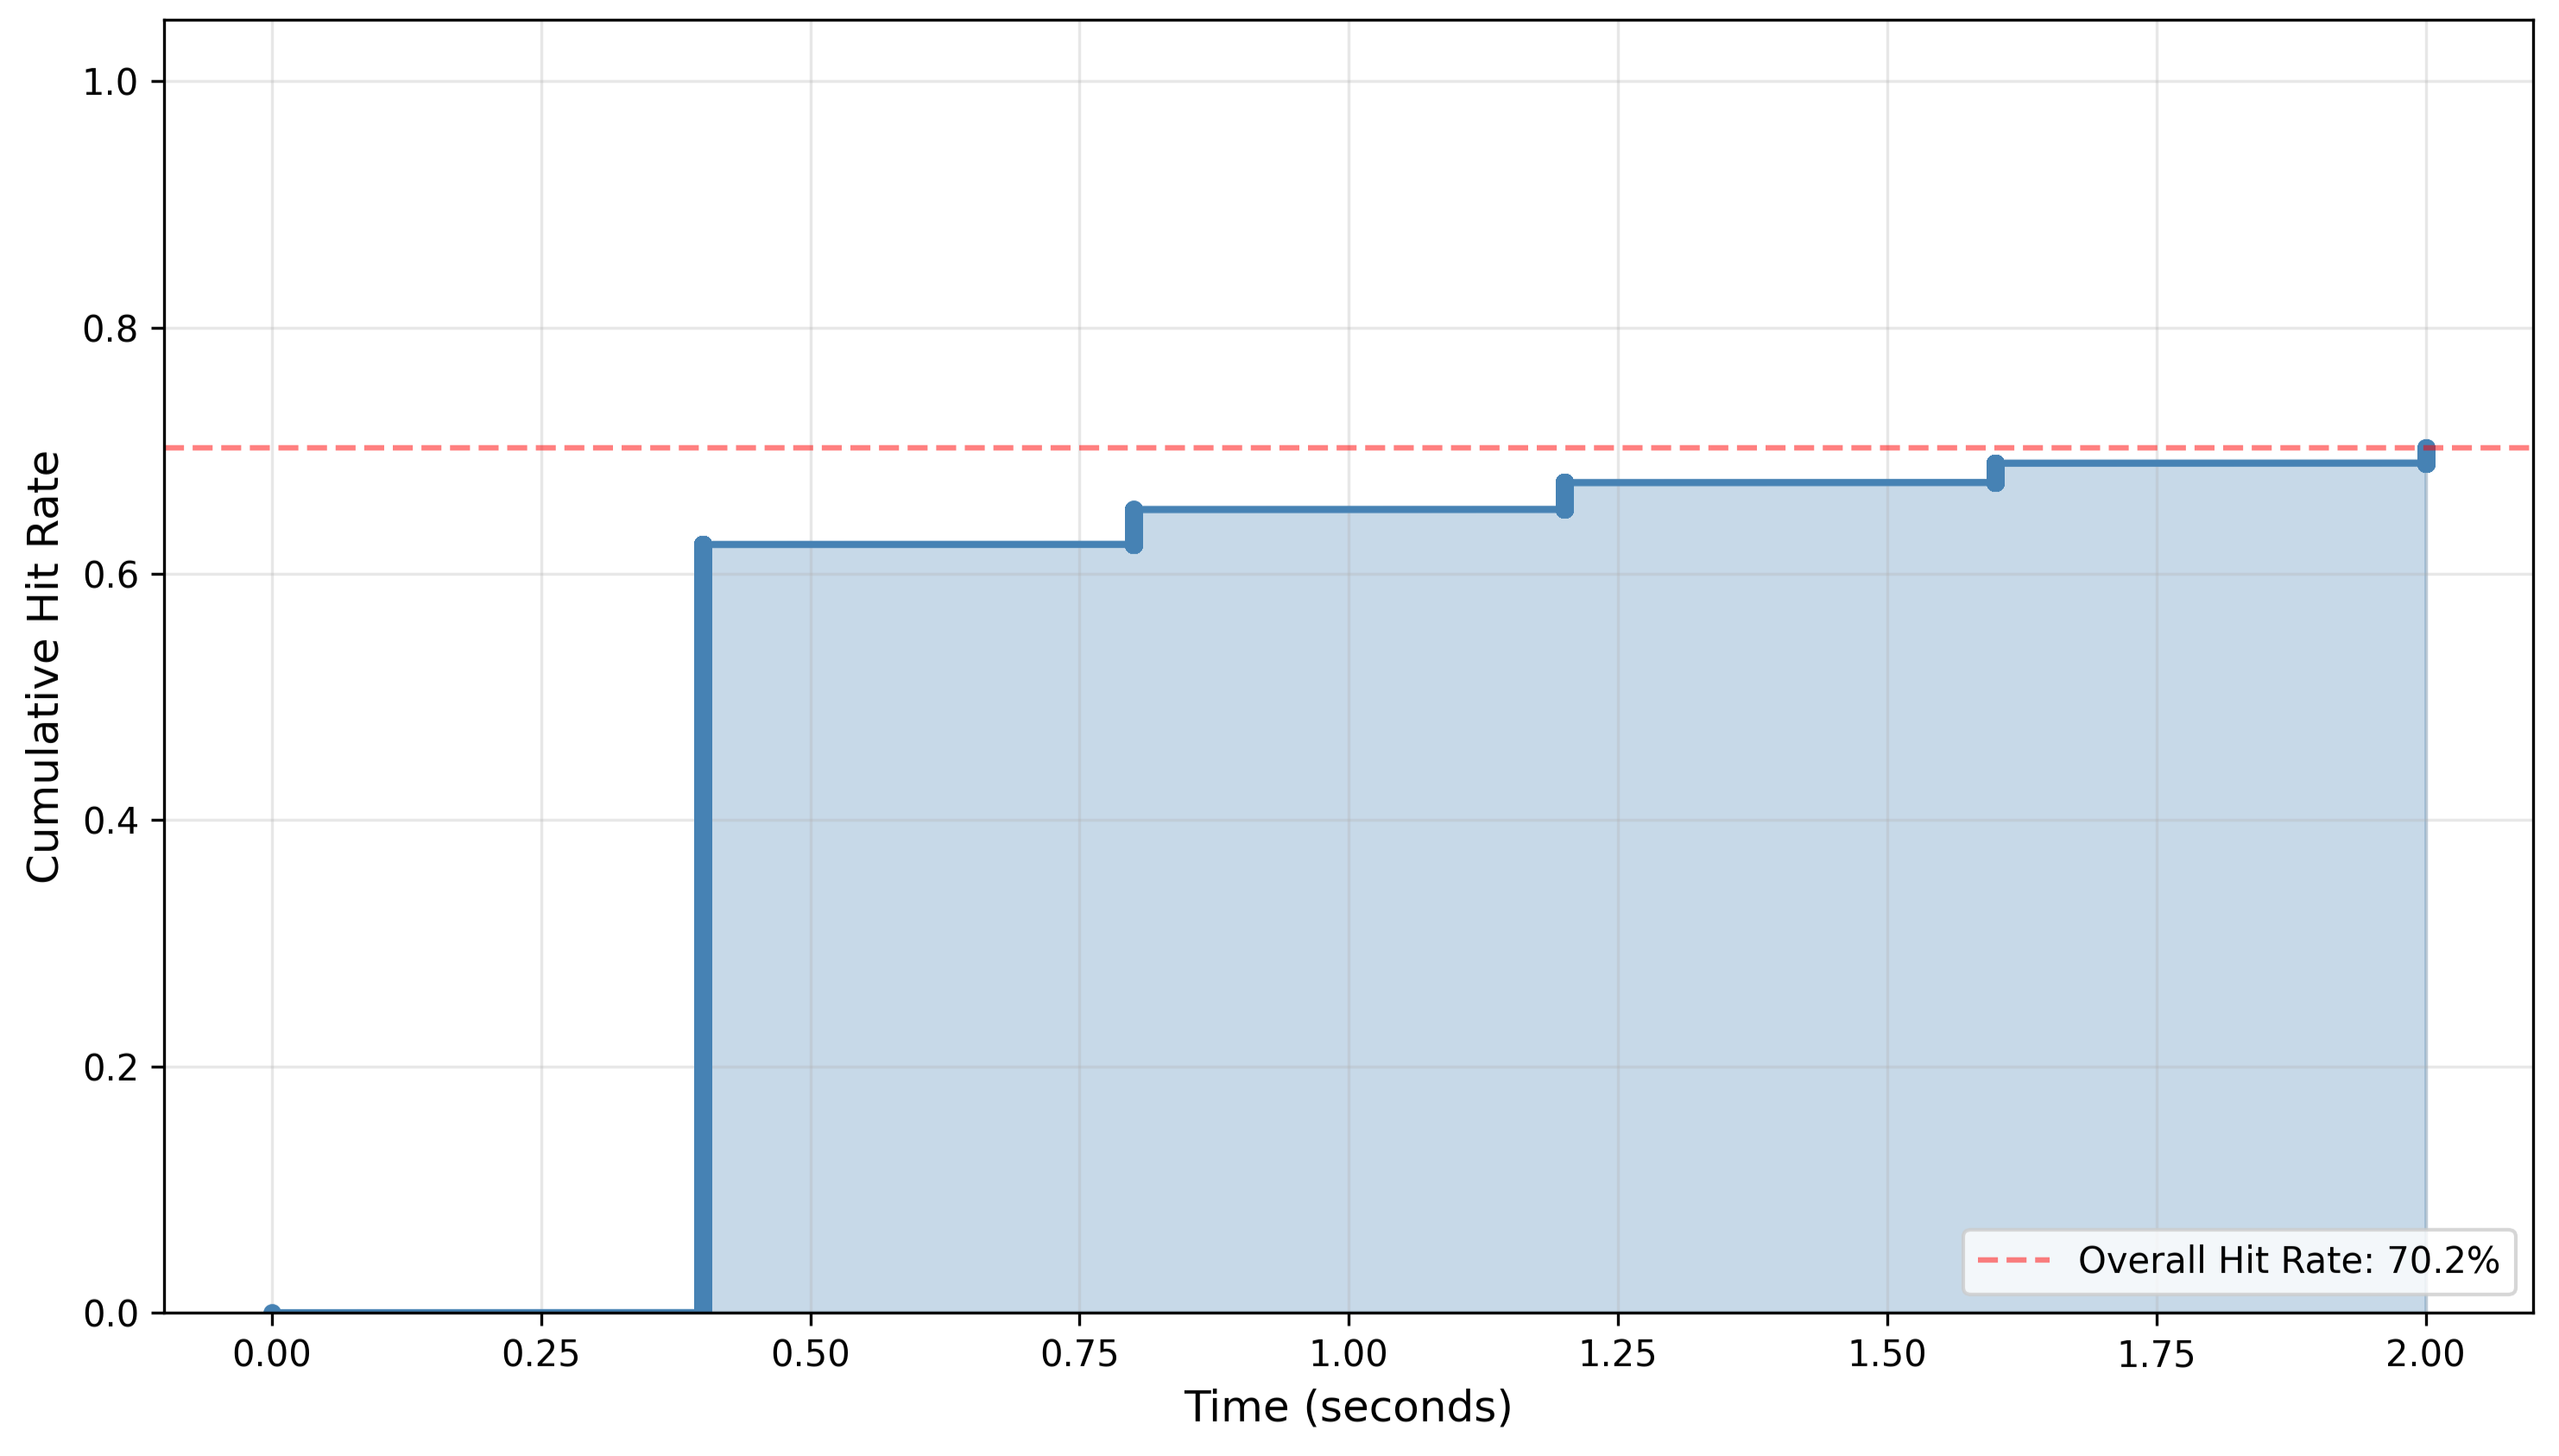
\includegraphics[width=\textwidth]{images/cumulative_hit_rate_grouped.png}
        \caption{Cumulative hit rate}
        \label{fig:cumulative_hit_rate_grouped}
    \end{subfigure}
    \hfill
    \begin{subfigure}[b]{0.49\textwidth}
        \centering
        
\includegraphics[width=\textwidth]{images/hit_count_summary_grouped.png}
        \caption{Hit/miss summary}
        \label{fig:hit_count_summary_grouped}
    \end{subfigure}
    \caption[Grouped horizon prediction results]{Grouped horizon prediction results within the 2\,s forecast horizon.}
    \label{fig:horizon_grouped}
\end{figure}

\par Overall, the selected \ac{DBN} is more reliable as a probabilistic short-horizon maneuver predictor than as a strict fine-grained next-step classifier.



\subsection{Computational Efficiency}
To assess the practical feasibility of the selected \ac{DBN} for online use, a latency benchmark was carried out on both CPU and GPU. 
The benchmark was performed on a Linux system with Python 3.11 and PyTorch 2.9.1, using an AMD Ryzen 9 7950X 16-Core CPU and an NVIDIA GeForce RTX 4090 GPU. 
Two settings were considered: a core \textit{update+predict} pipeline that operates directly on window-level observations, and an end-to-end 
\textit{frame$\rightarrow$window$\rightarrow$predict} pipeline that also includes online window construction.

\par For the present framework, the end-to-end latency is especially relevant. 
Since the dataset is sampled at 25\,Hz and a new window is issued every 10 frames, a new prediction is required every 0.4\,s (400\,ms). 
The measured steady-state runtimes are far below this limit, as summarized in Table~\ref{tab:latency_benchmark}.
\begin{table}[htbp]
\centering
\caption{Mean steady-state latency of the selected model for different settings.}
\label{tab:latency_benchmark}
\begin{tabular}{llcc}
\toprule
Pipeline & Mode & CPU [ms] & GPU [ms] \\
\midrule
window$\rightarrow$predict & Single vehicle & 0.1642 & 6.0960 \\
window$\rightarrow$predict & Batched ($B=5$ vehicles) & 0.2096 & 0.5483 \\
window$\rightarrow$predict & Sequential ($B=5$ vehicles) & 0.7957 & 15.8495 \\
frame$\rightarrow$window$\rightarrow$predict & Single vehicle & 0.5728 & 8.4220 \\
frame$\rightarrow$window$\rightarrow$predict & Batched ($B=5$ vehicles) & 1.9084 & 13.1136 \\
frame$\rightarrow$window$\rightarrow$predict & Sequential ($B=5$ vehicles) & 2.6668 & 33.3626 \\
\bottomrule
\end{tabular}
\end{table}


\par For the practically most relevant end-to-end case, a single online prediction requires only about $0.57\,\mathrm{ms}$ on CPU. 
Even when five input streams are processed together in batched mode, the total runtime is only about $1.91\,\mathrm{ms}$ on CPU, 
which remains far below the available 400\,ms decision interval. 
This indicates that the proposed framework is easily fast enough for real-time short-horizon prediction.

\par The batched results also show that parallel processing of multiple streams is feasible. 
Compared with a simple sequential loop over five streams, batching reduces the window-only runtime from about $0.80\,\mathrm{ms}$ to $0.21\,\mathrm{ms}$ on CPU, and from about $15.85\,\mathrm{ms}$ to $0.55\,\mathrm{ms}$ on GPU. 
For the end-to-end case, batching reduces the runtime from about $2.67\,\mathrm{ms}$ to $1.91\,\mathrm{ms}$ on CPU, and from about $33.36\,\mathrm{ms}$ to $13.11\,\mathrm{ms}$ on GPU. 
Thus, if predictions for several vehicles must be produced at the same time, the batched implementation is the more efficient choice.

\par The selected \ac{DBN} is compact, so fixed GPU overheads dominate the total latency in the low-batch regime. These overheads are less visible only 
in the batched \textit{window$\rightarrow$predict} case, where the frame-to-window preprocessing is bypassed and GPU parallelism can be utilized more effectively.

\par For the model used in this work, CPU execution is generally more favorable than GPU execution in the low-batch online regime. 
Although the GPU can accelerate the batched \textit{window$\rightarrow$predict} case, it is slower in the more realistic end-to-end setting considered here. 
Overall, the latency benchmark leads to three practical conclusions: \\
(i) real-time deployment is easily feasible because all measured end-to-end runtimes are far below the 400\,ms decision interval, \\
(ii) CPU is the preferred target for low-batch per-vehicle online inference, and \\
(iii) batching is still beneficial when many vehicles must be processed concurrently.

\section{Ablation Studies on Latent-State Cardinality}
This section examines how the performance of the proposed \ac{DBN} changes when the number of latent style and action states is varied. 
The selected reference model uses two style states and four action states. 
The ablation study has two goals. 
First, it tests whether three or five action states are more suitable than four when the two-style structure is kept. 
Second, it evaluates whether the style variable itself is necessary by comparing the reference model with variants that use only one style state.

\par The comparison is based on validation log-likelihood during training, test-set \ac{NLL}, effective occupied-state statistics, and semantic interpretability of the 
learned latent states. The occupancy-based quantity is used here only as a descriptive diagnostic and not as a model-selection criterion by itself.
Together, these results help assess whether the chosen latent-state cardinality provides a good balance between model flexibility and meaningful behavioral structure.
\begin{figure}[htbp]
    \centering
    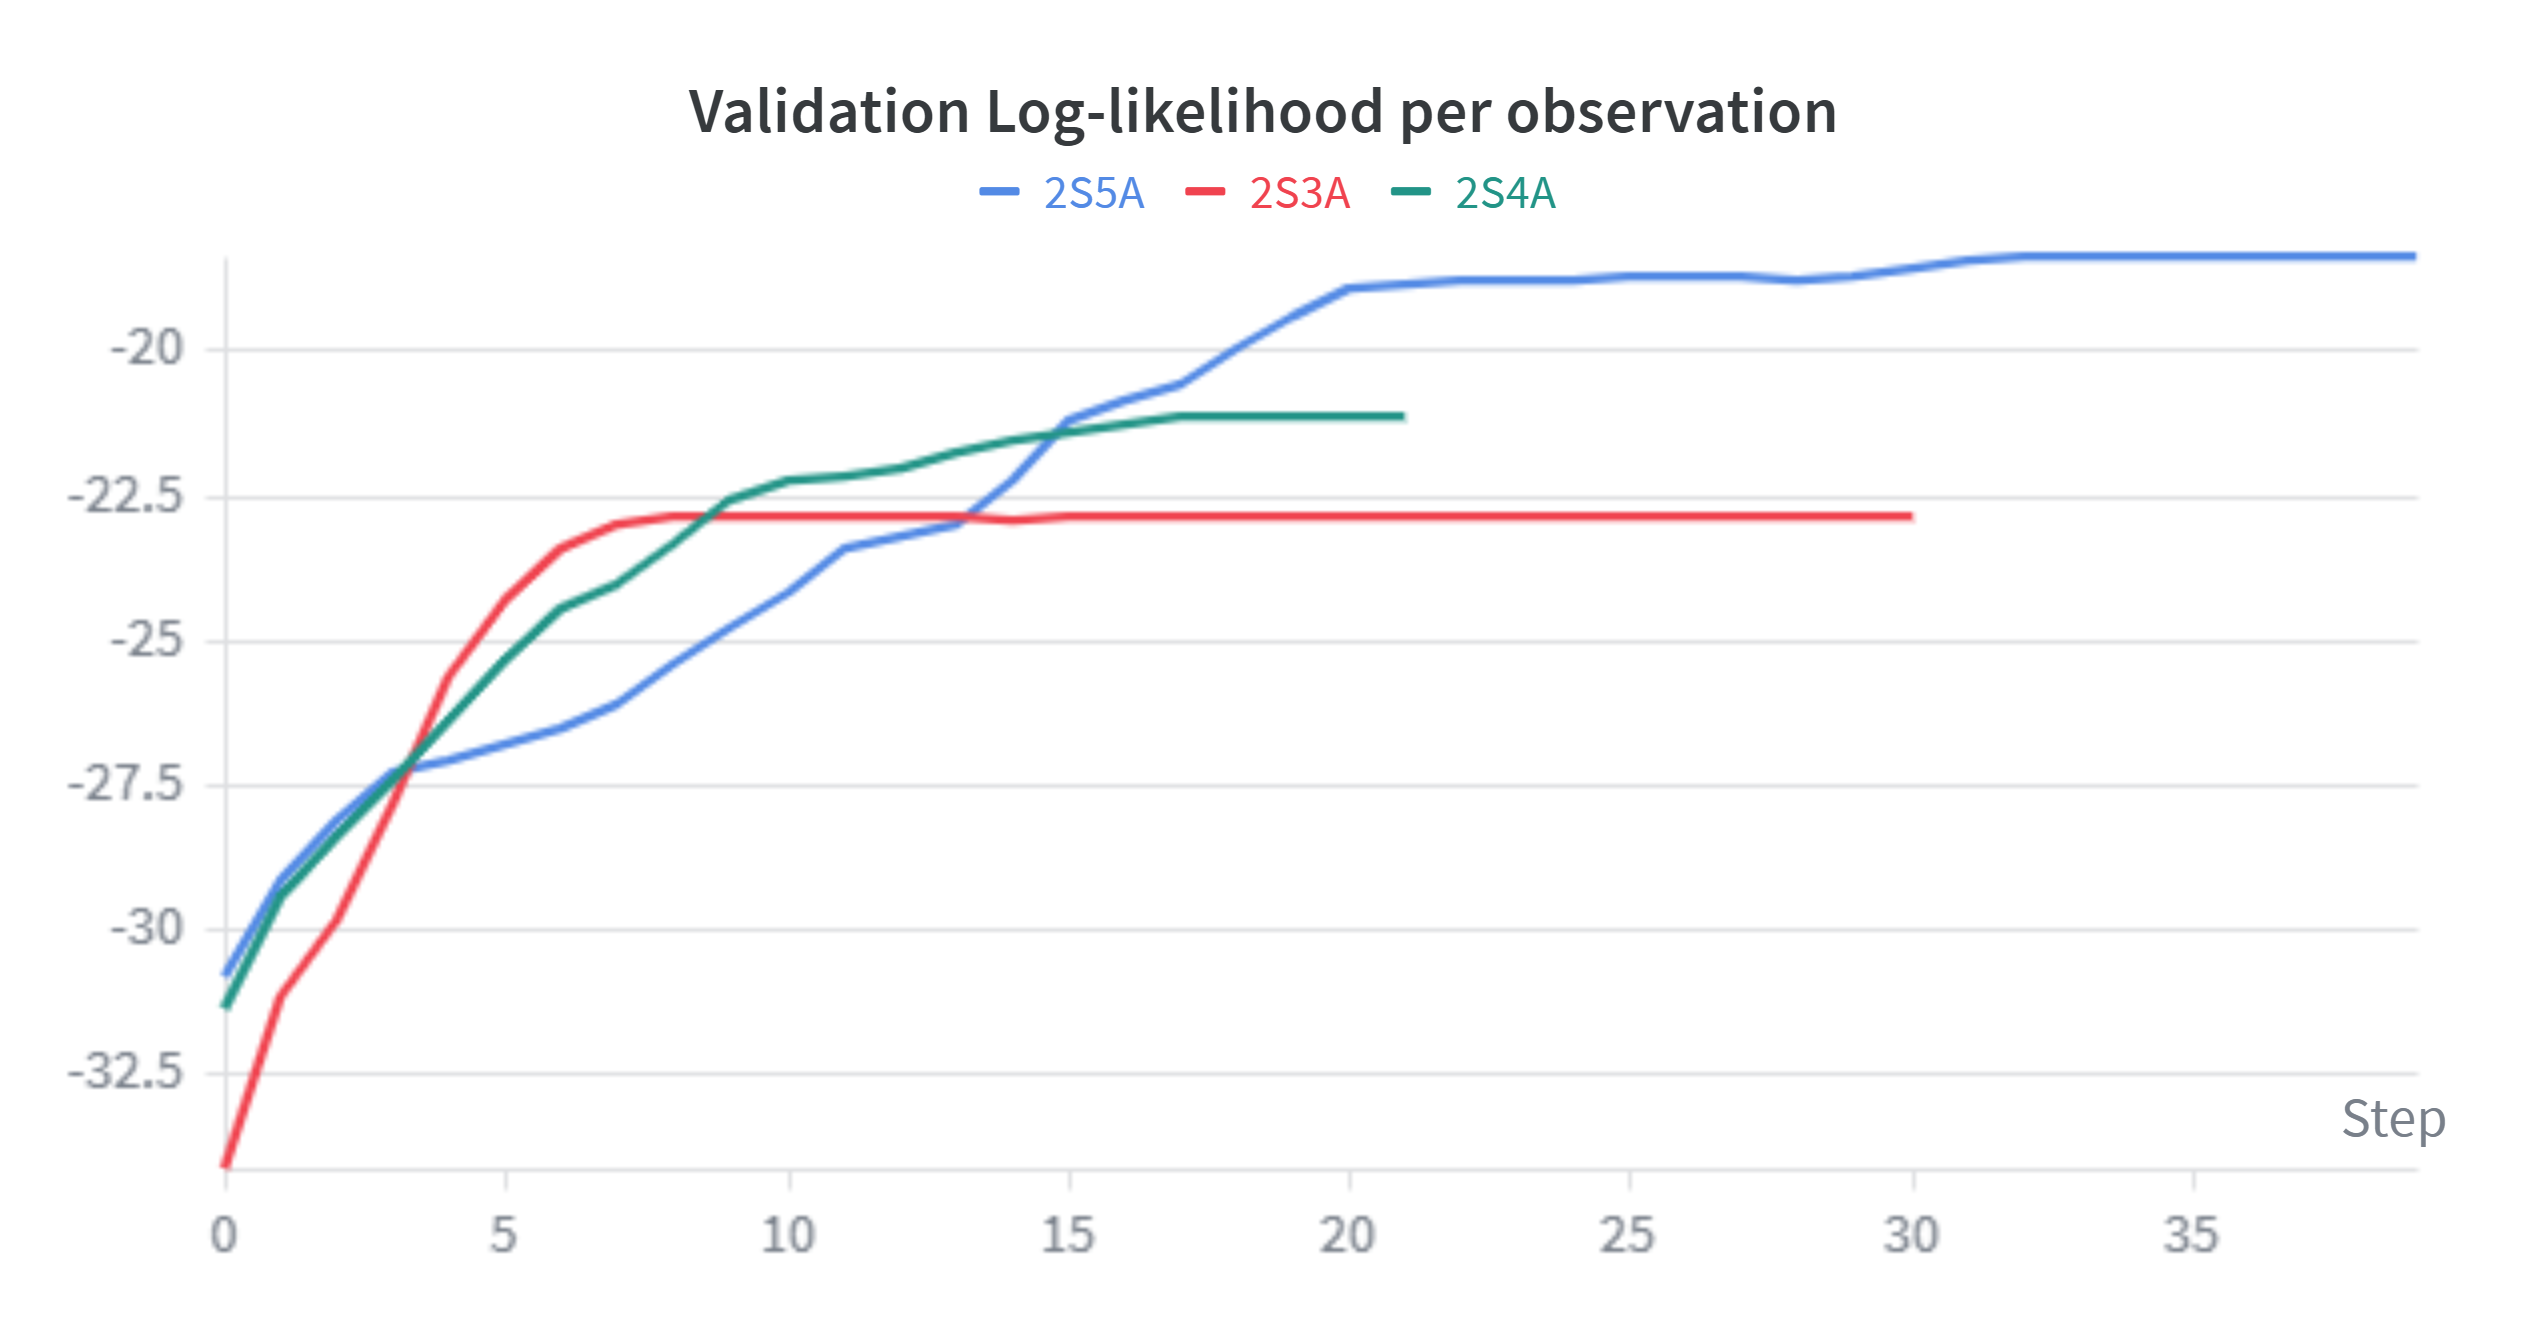
\includegraphics[width=0.95\textwidth]{images/val_ablation_two_style.png}
    \caption[Validation log-likelihood for two-style ablations]{Validation log-likelihood per observation for two-style models (2S3A, 2S4A, 2S5A).}
    \label{fig:val_ablation_two_style}
\end{figure}
\begin{figure}[htbp]
    \centering
    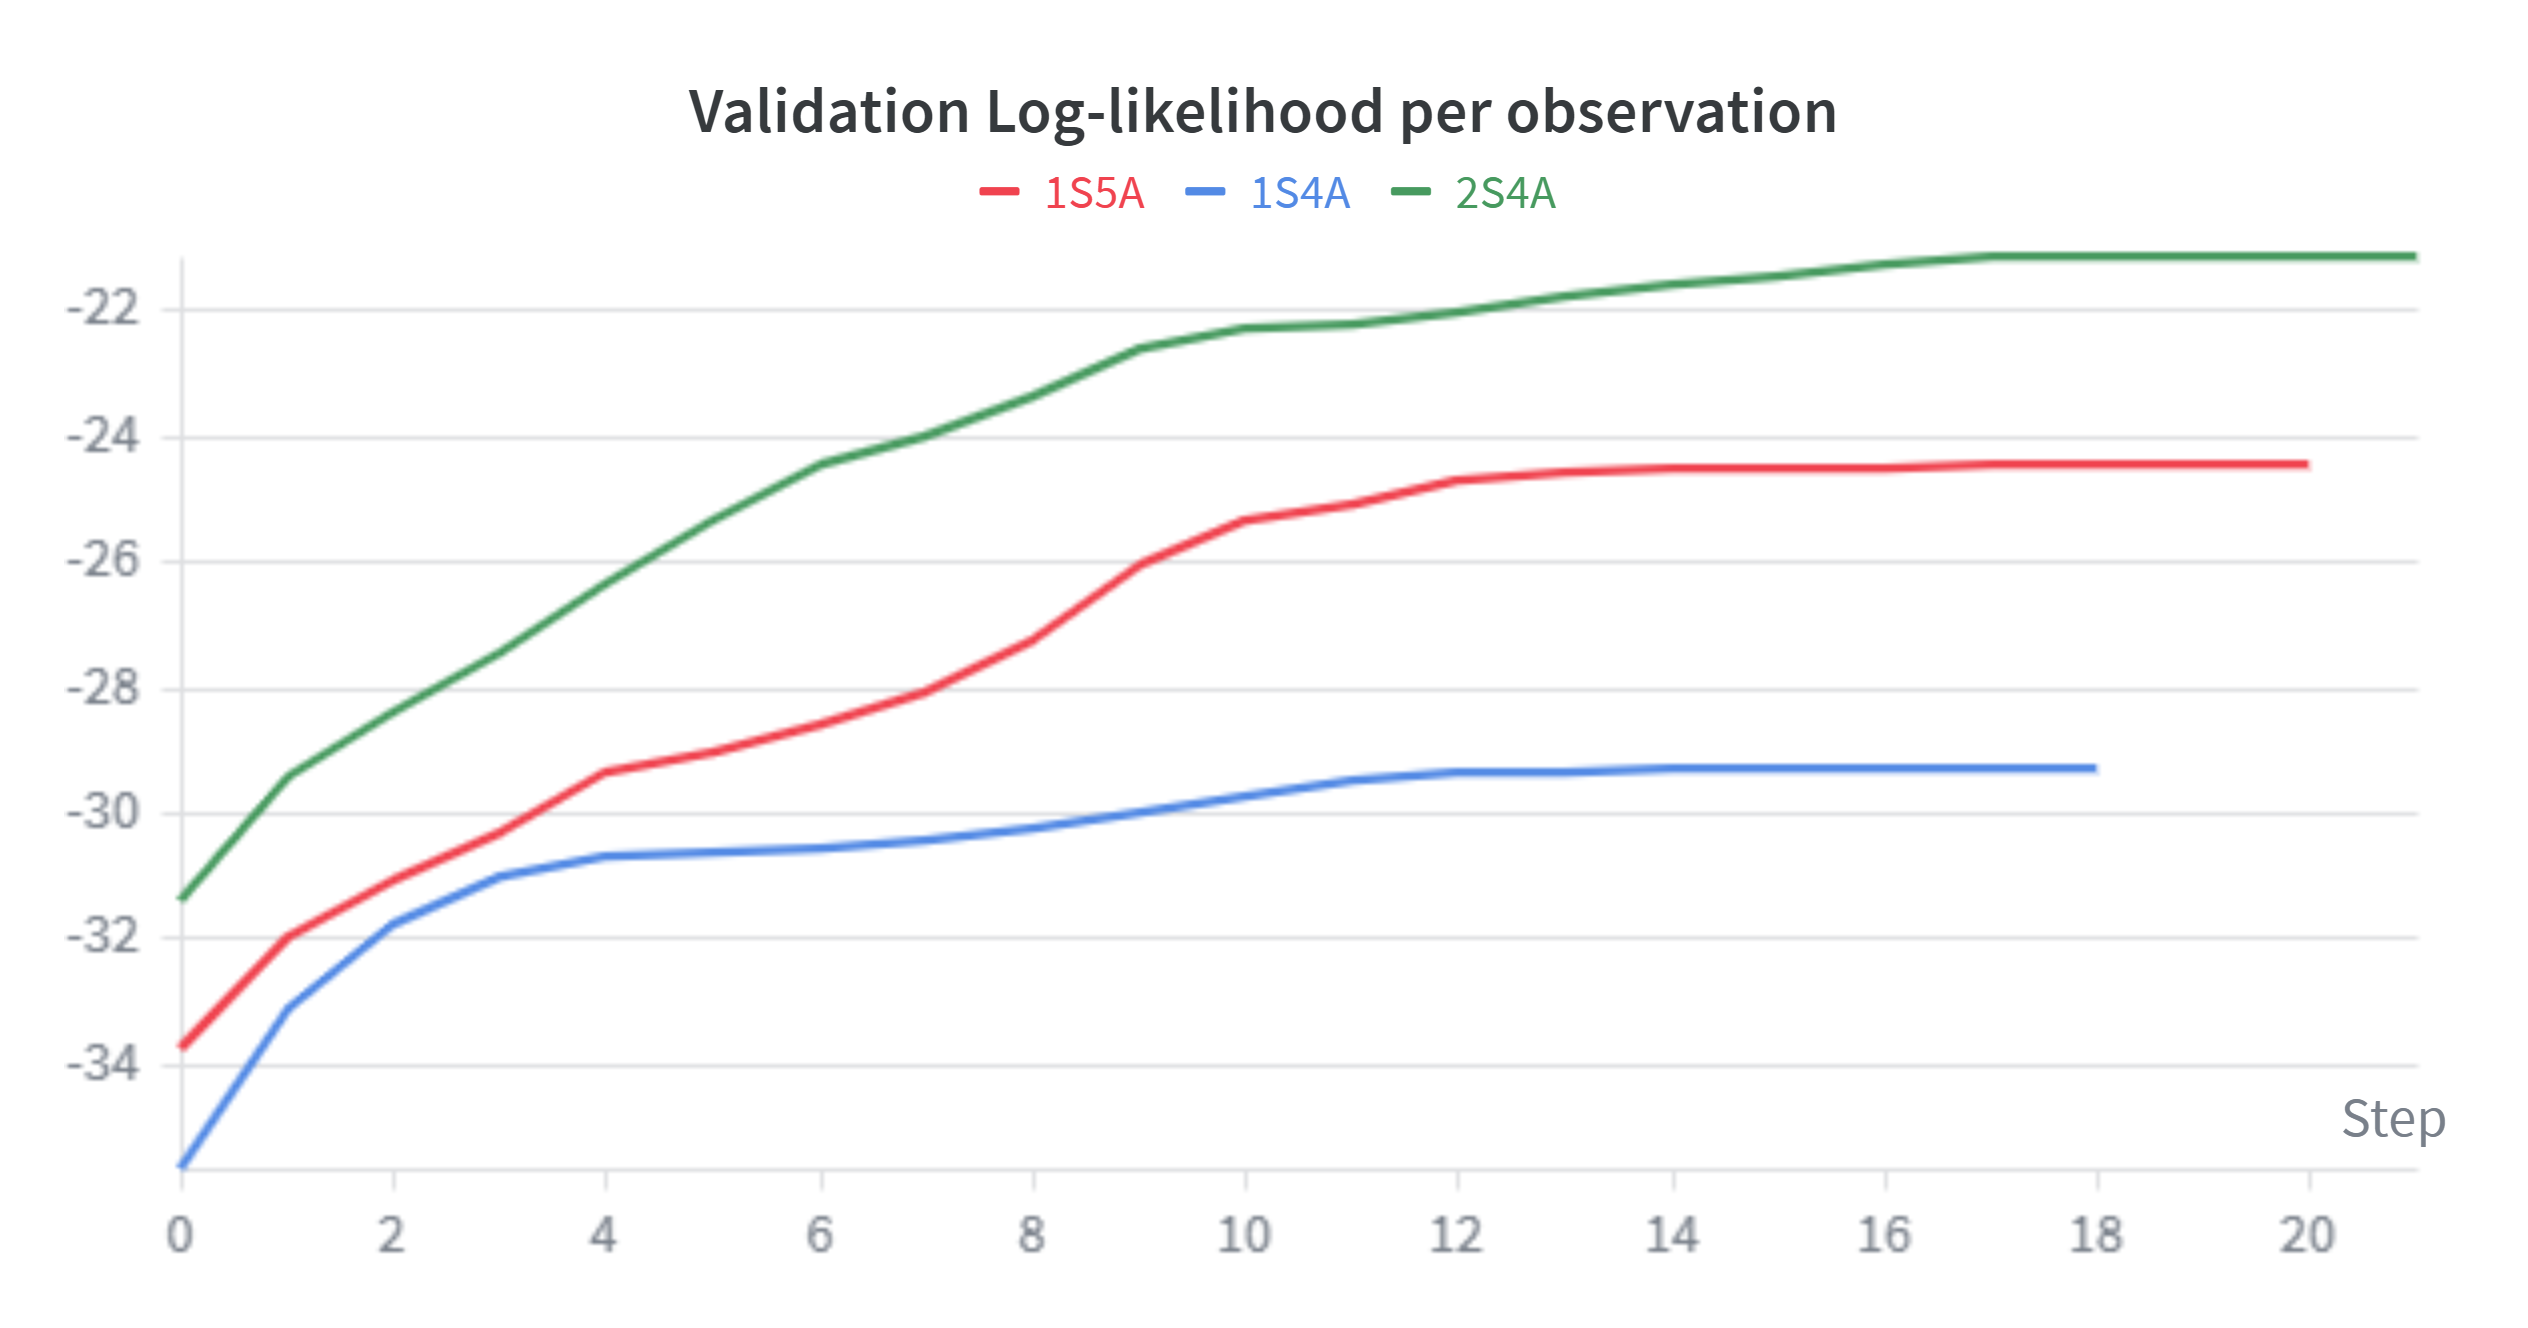
\includegraphics[width=0.95\textwidth]{images/val_ablation_one_style.png}
    \caption[Validation log-likelihood for one-style ablations]{Validation log-likelihood per observation for one-style models (1S4A, 1S5A) compared with the selected 2S4A reference.}
    \label{fig:val_ablation_one_style}
\end{figure}

\par Overall, the ablation results support the chosen latent-state design. 
Reducing the number of action states to three makes the behavioral partition too coarse, while removing the style variable causes a much larger drop in model quality. 
Increasing the number of action states can improve the fit, but it does not remove the need for a separate style latent. 
Taken together, these experiments show that the selected two-style, four-action structure provides a strong balance between performance, interpretability, and model complexity.


\subsection{Ablation with 2 Style States and 3 Action States}
The first ablation reduces the number of action states from four to three while keeping the two-style structure unchanged. 
This tests whether three action states are sufficient to capture the main maneuver patterns in the data.

\par Figure~\ref{fig:val_ablation_two_style} shows that the 2S3A model improves quickly during the early training iterations, but then saturates at a lower validation log-likelihood 
than the 2S4A model. 
Its validation performance levels off at about \(-22.8\) per observation, whereas the 2S4A model continues improving and reaches about \(-21.2\). 
This suggests that three action states are not enough to represent the full variation of the observed driver behavior.

\par The same pattern appears on the test set. 
The 2S3A model achieves a test \ac{NLL} of \(22.84\) per time step, which is worse than the selected 2S4A model. 
This confirms that the weaker validation performance also carries over to unseen data.

\par The occupied-state statistics show that this weaker result is not caused by state collapse. 
The model still uses almost all available action capacity, with an effective number of occupied joint states of about \(k_{\mathrm{eff}}^{\mathrm{joint}}=5.07\). 
This suggests that the limitation comes from insufficient action resolution rather than from unused latent states.


\par The semantic analysis further shows that the 2S3A model still learns meaningful latent states. 
The two style states remain interpretable, and the three action states still capture broad behavior categories such as following, acceleration-related behavior, 
and braking-related behavior. 
However, the partition is coarser than in the 2S4A case. 
Some patterns that are more clearly separated in the selected model are merged into the same action state here.  
In other words, the model still works, but the action semantics are less distinct.

\par This result indicates that three action states are not sufficient for the desired level of behavioral separation. 
The fourth action state in the selected model therefore appears useful rather than redundant.


\subsection{Ablation with 2 Style States and 5 Action States}
The second ablation increases the number of action states from four to five while keeping two style states. 
This tests whether additional action capacity can further improve the model.

\par As shown in Figure~\ref{fig:val_ablation_two_style}, the 2S5A model reaches the best validation log-likelihood among the evaluated two-style variants. 
Its validation curve continues improving beyond both 2S3A and 2S4A and finally reaches about \(-18.4\) per observation. 
On the test set, it achieves a test \ac{NLL} of \(18.33\) per time step. The occupied-state statistics further show that the additional capacity is actively used, 
with \(k_{\mathrm{eff}}^{\mathrm{joint}}=7.99\).
Numerically, this is the strongest result among the tested action cardinalities.

\par The semantic analysis also shows that the extra action state is not wasted. 
The model separates a richer set of action patterns, including lane-change-related behavior, steady following, stronger acceleration, braking, and gentler acceleration. 
In the more interaction-dominant style, it also isolates more critical braking and stop-and-go-like acceleration behavior. 
This means that the additional action state is used to create a finer behavioral partition rather than simply duplicating existing states.

\par However, this finer partition is not automatically preferable for the final model choice. 
For the objectives of this thesis, high likelihood alone is not sufficient; the learned maneuver taxonomy should also remain compact and stable.
In the 2S5A setting, several action states become very specific sub-variants of similar maneuvers. 
This increases semantic complexity and reduces the clarity of the resulting labels. 
The 2S4A model therefore remains the selected reference because it provides a better trade-off between predictive performance, 
interpretability, and actionable maneuver grouping.


\subsection{Ablation with 1 Style State and 4 Action States}
The next ablation removes the style hierarchy completely by using only one style state and four action states. 
This model tests whether the style variable is truly needed, or whether all relevant behavior can be represented through action states alone. 

\par The result is clearly worse than in the two-style setting. 
Figure~\ref{fig:val_ablation_one_style} shows that the 1S4A model remains far below the 2S4A model throughout training. 
Its validation log-likelihood saturates near \(-29.3\) per observation, whereas the selected 2S4A model reaches about \(-21.2\). 
This large gap shows that removing the style latent strongly reduces model quality.   

\par The same pattern is visible on the test set. 
The 1S4A model achieves a test \ac{NLL} of \(28.30\) per time step, which is substantially worse than the two-style model. 
Again, the poor result cannot be 
explained by unused action states. 
The model still occupies nearly all available action capacity, with \(k_{\mathrm{eff}}^{A}=3.92\).
Thus, the performance drop is not limited to training or validation, but also appears on the held-out test set.

\par The semantic analysis helps explain this result.   
Even without a style latent, the model still learns action states that roughly correspond to acceleration, braking, and stable following. 
However, the remaining state becomes broader and less clean, combining freer motion, lane-change-related behavior, and lower interaction pressure from front neighbors. 
This suggests that, without a separate style variable, the action states must represent two different aspects at the same time: 
the short-term maneuver itself and the broader traffic regime in which the maneuver occurs.

\par This ablation therefore shows that the style variable is not just an additional modeling detail.  
It plays an important role in separating persistent interaction context from immediate maneuver dynamics. 
Without it, the action states become more entangled and the overall model fit deteriorates strongly.




\subsection{Ablation with 1 Style State and 5 Action States}

A final ablation was carried out with one style state and five action states. 
The purpose of this experiment is to test whether the loss of the style variable can be compensated for by adding one more action state.

\par Compared with the 1S4A model, the 1S5A model performs clearly better. 
Its validation curve in Figure~\ref{fig:val_ablation_one_style} rises well above the 1S4A curve and reaches about \(-24.4\) per observation. 
On the test set, it achieves a test \ac{NLL} of \(24.31\) per time step. The occupied-state statistics show that the additional action 
capacity is partly used, with \(k_{\mathrm{eff}}^{A}=4.06\). 

This is a clear improvement over the 1S4A model, which means that the extra action state is useful.

\par The semantic analysis shows that the added action state improves the behavioral partition compared with with the 1S4A case. 
In particular, braking, stable following, and acceleration appear more clearly as separate action states. 

\par However, the separation is still not fully clean. 
Some states, especially those related to lane-change and low-speed adjustment behavior, still reflect more than one factor at the same time. 
For example, they are shaped not only by whether the vehicle is changing lane or adjusting speed, but also by lateral motion, nearby vehicles in 
adjacent lanes, front-vehicle presence, and the current speed level. 
This means that the action states still absorb part of the surrounding interaction context instead of representing only the maneuver type. 
Thus, adding more action states can reduce semantic mixing, but cannot eliminate it as long as no separate style latent is present. 





